\documentclass{article}
\usepackage[utf8]{inputenc}
\usepackage[round]{natbib}
\usepackage[colorlinks=true, citecolor=blue]{hyperref}
\usepackage[T1]{fontenc}
\usepackage[french,english]{babel}
\usepackage{textcomp}
\usepackage{verbatim}
\usepackage{amsmath}
\usepackage{amssymb}
% \usepackage{booktabs}
\usepackage{threeparttable}
% \usepackage{hyperref}
\usepackage{lscape}
\usepackage{pifont}
\newcommand{\cmark}{\ding{51}}
\newcommand{\xmark}{\ding{55}}
\usepackage{chngpage}
\usepackage{array}
\usepackage{multirow}
\usepackage{graphicx}
\usepackage[export]{adjustbox}
\usepackage{float}
\usepackage{geometry}
\usepackage{booktabs,multirow,makecell}
\usepackage{tabularx}
\usepackage{tikz}
\usetikzlibrary{calc,positioning,fit}
\usepackage{xcolor}
\geometry{hmargin=3.5cm,vmargin=2.5cm}
\usepackage[justification=centering]{caption}
\usepackage[version=4]{mhchem}
\title{Role of forest biomass in the Finnish decarbonisation\footnote{PhD student at University of Pisa}\footnote{mail. m.bordenave@student.unisi.it}\footnote{\url{https://orcid.org/0000-0002-5571-5877}}}
\author{Matthieu Bordenave}
\date{}

\begin{document}

\maketitle{}
\begin{abstract}
Forest biomass supplies around 25\% of Finland's primary energy, yet most whole-energy system models treat it as a homogeneous, unconstrained resource -- an assumption that ignores real biodiversity ceilings, carbon-sink constraints, and physical disturbance risks. This paper presents the application of EnergyScope TD, an open-source linear-programming whole-energy system model, to Finland, and uses it to examine how contrasting forest-management choices propagate into 2035 decarbonisation pathways. Three contributions are made: a model validation against the 2017 observed energy balance (primary-energy aggregates, electricity mix, and net CO$_2$ emissions reproduced within approximately 5\% on most indicators); the translation of three forest-management narratives -- intensive (S1), balanced (S2), and conservation-first (S3) -- into differentiated stepwise biomass supply curves; and the analysis of a completed 2035 scenario matrix crossing these narratives with GHG targets. Under the $-95\%$ target, the conservation scenario saturates its 40~TWh domestic ceiling and becomes the highest-cost configuration, as the optimiser must substitute or accept expensive imports once the biodiversity constraint eliminates all intermediate domestic steps. Forest-biomass governance choices therefore materially shape both the feasibility and cost of deep decarbonisation. This work is a deliberate first step toward a broader physical-risk research agenda in which climate-driven disturbance shocks -- bark beetle outbreaks, windstorms, compound events -- will be layered onto these management baselines.
\end{abstract}

\noindent\textbf{Keywords:} Finland; EnergyScope TD; forest biomass; decarbonisation; energy system optimisation.

\newpage

\section{Introduction}


Finland's pathway to deep decarbonisation sits at the intersection of three system constraints: electrifying end uses at scale, integrating high shares of variable renewables with adequate storage and flexibility, and managing a uniquely large forest biomass resource under increasing scrutiny about carbon accounting and biodiversity impacts. Forests cover roughly 75\% of Finland's land area, and woody biomass already supplies around 25\% of national primary energy -- largely through industrial residues, logging by-products, and combustion in district heat and combined heat-and-power (CHP) plants -- making the forest sector structurally embedded in both the energy system and the wider bioeconomy \citep{blattertSectoralPoliciesCause2022}. In this context, energy planning tools are not only asked to identify least-cost technology mixes, but also to make explicit cross-sector trade-offs between electricity, heat and mobility, and the role of renewable fuels and carbon capture options where direct electrification is difficult.

A common thread in European decarbonisation narratives is a strong reliance on forest biomass as a flexible, dispatchable, and storable renewable resource able to bridge the gap between electrification and residual uncompressible CO2 emissions. Finland's own Bioeconomy Strategy exemplifies this bet: it frames the forest as a cornerstone of both climate policy and industrial competitiveness by setting ambitious targets for roundwood mobilisation and high-value bio-based products. Yet this narrative sits in tension with two other imperatives that pull in opposite directions. First, biodiversity safeguards impose a real ceiling on what can actually be harvested: \citet{monkkonenEcologicallyEconomicallySustainable2024} show that current timber harvesting in southern Finland already approaches the maximum economically sustainable level (roughly 96\% of the mean annual increment), while an ecologically sustainable safe operating space -- one that maintains favourable habitat conditions for boreal forest species under the IUCN Red List of Habitats framework -- would require reducing harvest to approximately 60\% of that ceiling. Second, physical risks amplified by climate change are making the supply itself increasingly uncertain: warming and drying trends are increasing the frequency and severity of windstorms, bark beetle outbreaks, and wildfires, all of which can alter the volume, quality, and spatial distribution of available biomass in ways that static supply assumptions cannot capture.

This paper develops a national application of EnergyScope TD to the Finnish energy system. EnergyScope TD is an open-source, linear programming, whole-energy system model that optimises both investment and operation for a target year, with an hourly representation through a typical-days reduction. This makes it suitable for scenarios with high penetration of intermittent renewables and storage \citep{limpensEnergyScopeTDNovel2019,limpensEnergyScopePathwayOpensource2024}. By construction, it provides an open-source and computationally efficient framework for exploring alternative transition constraints.

Methodologically, the first contribution is to build and document a Finland-specific dataset and calibration for a 2035 snapshot analysis, consistent with EnergyScope TD requirements (end-use demands, technology portfolio, resource potentials, and time series for key variables). The second contribution is model verification through historical reproduction. Following the approach used for Switzerland and Belgium, we constrain the model with observed end-use demands and technology shares for a past reference year and compare model outputs to reported energy balances and emissions, as a practical test of the model's ability to represent a national system \citep{moretCharacterizationInputUncertainties2017,thiranExploringOptionsFossilfree2025,limpensGeneratingEnergyTransition2021}. The third contribution is the construction of differentiated biomass supply curves for Finland under three contrasting forest-management narratives: intensive (bioeconomy-aligned), balanced, and conservation (biodiversity-first). Following the stepwise methodology of \citet{collaOptimalUseLignocellulosic2022}, each narrative is translated into a set of biomass availability steps differentiated by feedstock origin, quality, and marginal cost. The purpose is threefold: to make explicit how competing societal choices about forest management propagate into the energy system; to quantify the cost of biodiversity safeguards in terms of system cost and decarbonisation difficulty; and to build a modelling foundation that can, in subsequent work, absorb disturbance-driven supply shocks as perturbations on top of these management baselines.

The overarching question motivating this research agenda is: how do physical constraints on boreal forests -- whether structural, from management regimes, or episodic, from natural disturbances -- affect the availability and cost of woody biomass, and through that, the economic competitiveness and decarbonisation trajectory of the Finnish energy system? Answering this question in full requires coupling forest dynamics and disturbance models with an energy system optimisation model. The present paper is a deliberate first step: it establishes the management-scenario baselines by studying how different forest-governance choices translate into the energy mix under a 2035 horizon. Subsequent work will layer disturbance shocks -- bark beetle outbreaks, windstorms, and compound events -- onto these baselines to study how physically induced wood price shocks and supply disruptions propagate through the energy sector. This question is particularly relevant because many whole-energy system models wrongly treat biomass as carbon neutral and with unlimited availability, which can strongly distort optimal outcomes in biomass-rich countries such as Finland.

The specific research questions addressed in this paper are:

\begin{enumerate}
  \item \textbf{Model credibility:} To what extent can a constrained EnergyScope TD setup reproduce Finland's observed energy balances and combustion emissions for a past reference year (within acceptable error margins), providing confidence for forward-looking scenario analysis?
  \item \textbf{Biomass supply and management narratives:} How do contrasting forest-management scenarios -- from intensive bioeconomy-aligned harvesting to biodiversity-constrained conservation -- translate into differentiated supply curves, and how much forest biomass is allocated across heat, power, industry and transport under each narrative?
  \item \textbf{Constraint interaction:} How do tighter forest-biomass ceilings interact with a -95\% GHG target, or with a nuclear phase-out and what cost penalty emerges when forest biomass can no longer act as a flexible adjustment margin?
\end{enumerate}

The remainder of the paper is organised as follows. Section~\ref{sec:lit_context} reviews the closest literature and the broader modelling context. Section~\ref{sec:model_description} describes the Finnish EnergyScope TD implementation, the main data inputs, and the qualification of the 2035 forest-biomass scenarios and supply curves. Section~\ref{sec:results} presents the 2017 validation, the 2035 scenario results, and the disturbance-shock extension that follows from the present modelling boundary. Section~\ref{sec:conclusion} concludes.

\section{Literature and context}
\label{sec:lit_context}

\subsection{Forest Management Scenarios, Physical Risks, and Remaining Gap}

The central challenge this paper engages with is the contested nature of Finland's forest biomass: an abundant and structurally embedded resource whose future availability depends both environmental conditions and forest management choices. \citet{blattertSectoralPoliciesCause2022} show that Finland's Bioeconomy Strategy, National Forest Strategy, and Biodiversity Strategy imply markedly different management mixes and ecosystem-service outcomes, revealing that forest biomass is not a neutral physical input but the product of conflicting policy priorities. \citet{ratyEUWoodProduction2023} examine directly whether EU wood production and biodiversity goals can be reconciled within Finnish forest policy and find that the trade-offs are substantial: integrated management cannot simultaneously satisfy all three pillars of wood mobilisation, carbon sinks, and biodiversity. \citet{monkkonenEcologicallyEconomicallySustainable2024} sharpen this point by arguing that current harvesting in southern Finland already approaches the maximum economically sustainable level, while an ecologically sustainable safe operating space -- one that maintains favourable habitat conditions under the IUCN Red List of Habitats framework -- would require a drastic reduction to roughly 60\% of that ceiling, with a fundamentally different balance between protection and intensive management. In a country this richly endowed in forest resources, the question is therefore not simply how much wood exists, but which forest system society is willing to legitimate.

At the European scale, regulatory pressure amplifies these domestic tensions. The EU Biodiversity Strategy for 2030 (EUBDS), which mandates strict protection of 10\% of EU forests and closer-to-nature management for an additional 20\%, has been modelled to reduce EU roundwood production by up to 48\% under intensive protection scenarios, with 50--73\% of this deficit compensated by increased imports from non-EU countries with weaker forest governance -- shifting rather than reducing global pressure on biodiversity \citep{fischerLeakageBiodiversityRisks2024,schierAssessmentPossibleProduction2022,kallioPotentialImpactsEUs2025,rosaCanForestManagement2023}. Policy safeguards such as deforestation-free supply chain regulations offer only partial mitigation unless sustainability criteria are enforced globally \citep{fischerLeakageBiodiversityRisks2024,zamaniDeforestationfreeTradeImpact2026}. For Finland -- one of Europe's largest roundwood producers -- these EU-level dynamics add a regulatory dimension to the domestic trade-off but do not resolve it.

A distinct and growing constraint on biomass availability comes from physical disturbances. There is now strong evidence linking climate change to an increasing frequency and severity of forest disturbances -- storms, pest outbreaks, fires, and droughts -- across the boreal and temperate zones \citep{andereggClimateRiskAnalysis2022b,lecina-diazCharacterizingForestVulnerability2021b}. For Finland specifically, \citet{venalainenClimateChangeInduces2020} identify wind as the dominant abiotic damage agent in Finnish boreal forests and show that the shortening of the soil frost period -- which normally anchors tree roots -- is increasing windthrow susceptibility across the most productive southern stands. A key non-linearity compounds this risk: wind-damaged areas generate large volumes of weakened or dead trees that become ideal breeding substrate for bark beetles, directly coupling abiotic and biotic disturbances in potentially multi-year cascades. These events exhibit fat-tailed uncertainty distributions that make both occurrence and magnitude difficult to project reliably, and their economic consequences are asymmetric: disturbances can trigger a short-term surge in timber supply through salvage logging, but typically produce long-term declines in forest productivity as damaged cohorts fall out of productive rotations for decades.

The Czech bark beetle crisis provides the clearest recent illustration of this dynamic. Beginning around 2015, the Czech Republic experienced a severe outbreak of the spruce bark beetle (\emph{Ips typographus}), intensified by elevated temperatures and extended drought periods \citep{hlasnyDevastatingOutbreakBark2021}, with a documented transition from wind- to drought-driven outbreak dynamics. By 2019, salvage logging constituted 92\% of the nation's total timber harvest, amounting to 25.5 million cubic metres \citep{simunekNorwaySpruceForest2024}. The abrupt increase in supply led to market oversaturation and a consequent collapse in timber prices; despite the higher physical volume, the forestry sector incurred economic losses estimated at EUR 1.12 billion \citep{tothImpactsCalamityLogging2020}. The widespread destruction of mature spruce stands also raises long-term concerns for forest regeneration, carbon sequestration, and future timber availability, potentially undermining the role of forests in climate mitigation.

Translating such disturbances into their energy-system implications is rare in the literature. \citet{reckaRoleBiomassDecarbonisation2023} represent the closest methodological precedent: using a spatially enriched partial equilibrium framework for energy market, TIMES, disaggregated to NUTS3 regions in Czechia, they incorporate four bark beetle infestation scenarios into forward-looking decarbonisation pathways to 2050. Their headline finding is that the infestation does not durably alter aggregate decarbonisation trajectories -- the effect on the renewable energy share remains below 1.5 percentage points and dissipates after 2030, because carbon-sink dynamics (captured through LULUCF accounting) dominate over fluctuations in biomass energy availability. However, tighter ecological constraints on forest biomass increase overall system costs and worsen the prospects of meeting renewable energy targets, while restricting biomass to residential uses forces other sectors to substitute with natural gas. This asymmetry -- a modest aggregate disturbance effect but a real and persistent cost penalty from ecological constraints -- suggests that the design of the biomass supply envelope matters at least as much as the occurrence of a disturbance shock itself, and motivates modelling frameworks that can represent both in a whole-energy system context.

The gap is that these strands remain weakly connected. Energy-system studies close to our question generally treat biomass availability as an exogenous scenario input; forest-policy studies stop before whole-energy-system reallocation; and disturbance studies rarely enter national optimisation models as explicit biomass supply and price shocks. \citeauthor{reckaRoleBiomassDecarbonisation2023}'s study is a notable exception, but it addresses disturbance dynamics in a non-forest-rich country rather than the political construction of supply ceilings in a country where biomass is structurally central. This paper addresses the first part of that gap by translating contested Finnish forest-management narratives into explicit biomass supply ladders within EnergyScope TD and by testing their implications for a completed 2035 forest \(\times\) GHG scenario matrix. Disturbance shocks are not yet implemented, but the evidence above provides the rationale for treating them as the next extension of the framework rather than as a side issue.



\subsection{Energy system modelling context}
EnergyScope TD is a whole-energy system optimisation model designed for scenario analysis of regional or national energy transitions with high temporal resolution while keeping computational times compatible with extensive sensitivity and uncertainty analyses. In contrast with power-only optimisation tools, EnergyScope TD represents power, heating, mobility and non-energy demand such as ammonia within a single, energy balance framework. A central design choice is the use of a limited set of representative "typical days" (TDs) to approximate intra-annual variability, combined with a reconstruction mechanism that preserves inter-day storage and capacity dynamics.

This modelling choice responds to a broader pattern identified in the deep decarbonisation literature. Based on a review of European decarbonisation scenario studies, \citet{borasioDeepDecarbonisationRegional2022} highlight both the diversity of modelling practices and a recurrent trade-off between scope and tractability: many studies rely either on top-down approaches or on tools primarily centered on the power sector, while fewer frameworks represent sector coupling across power, heat and mobility in a consistent optimisation setting. This motivates the use of whole-energy system models that can capture cross-sectoral substitutions and flexibility needs while remaining sufficiently lightweight for systematic scenario exploration.

A key motivation for EnergyScope TD is therefore that combining (i) multi-sector coverage, (ii) open-source availability, (iii) endogenous system design and operation, and (iv) short runtimes is uncommon in large-scale energy planning practice. Table~\ref{tab:model-comparison} summarises this positioning using the comparative criteria reported in \citet{limpensEnergyScopeTDNovel2019}.

\begin{table}[t]
  \centering
  \renewcommand{\arraystretch}{1.15}
  \begin{tabularx}{\linewidth}{lcccc}
    \toprule
    \textbf{Model} & \textbf{Multi-sector} & \textbf{Open-source} & \textbf{Optimisation} & \textbf{Comp. time} \\
    \midrule
    Calliope        & \cmark & \cmark & \cmark & mins \\
    COMPOSE         & \cmark & \xmark & \cmark & - \\
    DESSTinEE       & \cmark & \cmark & \xmark & s \\
    DIETER          & \xmark & \cmark & \cmark & mins \\
    EnergyPLAN      & \cmark & \xmark & operation only  & s \\
    MARKAL/TIMES    & \cmark & \xmark & investment only & 5-35 min \\
    oemof           & \cmark & \cmark & \cmark & mins \\
    OSeMOSYS        & \cmark & \cmark & \cmark & mins \\
    PyPSA           & \cmark & \cmark & \cmark & mins \\
    STREAM          & \cmark & \xmark & \xmark & - \\
    Switch          & \xmark & \cmark & \cmark & 10-60 min \\
    URBS            & \xmark & \cmark & \cmark & 20 min \\
    \addlinespace
    \textbf{EnergyScope TD} & \textbf{\cmark} & \textbf{\cmark} & \textbf{\cmark} & \textbf{$\sim$1 min} \\
    \bottomrule
  \end{tabularx}
  \caption{Indicative comparison of large-scale energy planning models along four criteria commonly used in the energy optimisation model literature: multi-sector scope, open-source status, optimisation of both design and operation, and order-of-magnitude runtime per scenario. Adapted from the comparison reported in \citet{limpensEnergyScopeTDNovel2019}.}
  \label{tab:model-comparison}
\end{table}

EnergyScope TD is part of a broader open modelling family. Historically, EnergyScope was first developed with coarser temporal aggregation and later extended toward hourly resolution with TDs and seasonality in EnergyScope TD, and further toward multi-regional representations in EnergyScope Multi-Cell \citep{hernandezEnergyScopeMultiCellNovel2021,thiranExploringOptionsFossilfree2025,borasioDeepDecarbonisationRegional2022}.

A common critique of EnergyScope TD, also emphasised in reviews of deep decarbonisation modelling, concerns spatial representation. Single-node national models may abstract from intra-country congestion, regional renewable heterogeneity, and the location of flexible demand, which can matter when electrification and variable renewables expand rapidly \citep{borasioDeepDecarbonisationRegional2022,limpensEnergyScopePathwayOpensource2024}. In the Finnish case, however, a first-order single-region representation is arguably more defensible than in countries with multiple dense load centers, because population, most energy demand, and the bulk of industrial activity are concentrated in the South, where the main transmission backbone and urban heat loads are also located. This motivates using EnergyScope TD for the present Finnish application.


In climate-mitigation narratives, biomass is often framed as a renewable and flexible resource, yet estimates of its future contribution remain highly uncertain because they depend on the constraint set adopted, including sustainability rules, technical feasibility, land and biodiversity limits, and economic conditions. Under sustainability-oriented assumptions, \citet{beringerBioenergyProductionPotential2011} report a wide global range for bioenergy in 2050 (126--216~EJ), broadly consistent with other assessments that apply different constraint sets and therefore obtain markedly different potentials \citep{haberlGlobalTechnicalPotential2010,schuelerGlobalBiomassPotentials2013,searleReassessmentGlobalBioenergy2015,ieaBioenergyAnnualReport2023}. At present, biomass already constitutes a substantial fraction of renewable energy supply and is used predominantly for heat \citep{ieaKeyWorldEnergy2020,ieaBioenergyAnnualReport2023}. Looking forward, deep decarbonisation implies defossilising multiple sectors simultaneously, which can increase competition for lignocellulosic resources as they are called upon to provide not only heat and power but also transport fuels and carbon-based feedstocks for industry and chemicals \citep{daioglouCompetingUsesBiomass2015}. Hence, the key transition question is not only \emph{how much} biomass can be mobilised, but also \emph{where} it should be allocated across final needs once economy-wide greenhouse-gas constraints bind \citep{collaOptimalUseLignocellulosic2022}.

A central theme in the biomass literature is that pathway comparisons should be made at the level of delivered services rather than solely at the level of produced fuels. Substitution logics distinguish fuel-level substitution from energy-service substitution, where the avoided emissions depend jointly on conversion efficiencies and on the demand-side technologies that ultimately use the energy carrier \citep{wahlundIncreasingBiomassUtilisation2004}. In this view, conversion losses in biofuel production may be compensated if the carrier enables substantially more efficient end-use devices \citep{steubingHeatElectricityTransportation2012}. This mechanism becomes visible in whole-system optimisation: \citet{codinagironesAssessmentCO2Mitigation2018} compare woody-biomass conversion routes inside a national energy-system optimisation and show that biofuel pathways can outperform direct biomass combustion in avoided \ce{CO2} only when accompanied by a broader shift toward efficient end-use options (for instance heat pumps or battery electric vehicles).


Taken together, these insights motivate the use of whole-energy system optimisation frameworks that decide endogenously both (i) how much biomass to use and (ii) how to distribute it across heat, electricity, mobility fuels, and material uses, conditional on the rest of the energy system and on emissions constraints. In that spirit, \citet{collaOptimalUseLignocellulosic2022} implement a detailed lignocellulosic biomass representation in EnergyScope TD in Belgium and analyse how optimal allocations shift as GHG constraints tighten, providing a documented modelling base that can be transferred to new country contexts.

\section{Model description}
\label{sec:model_description}

This section presents the implemented Finnish EnergyScope TD setup, including the two-step temporal aggregation and optimisation workflow, the main national input data used to calibrate demand and supply, and the 2035 forest-biomass scenario qualification translated into supply curves.

\subsection{Two-step methodology and data flow}
EnergyScope TD is typically implemented as a two-step workflow:
(i) a temporal aggregation step that selects a small set of TDs (and their weights and sequence), and
(ii) a linear programming (LP) optimisation step that determines the least-cost (or otherwise constrained) energy system configuration for a target year under the TD representation \citep{limpensGeneratingEnergyTransition2021}.

The workflow therefore combines a temporal aggregation step and a system optimisation step. In practice, Step~1 selects representative days and reconstructs a chronological year, while Step~2 solves the least-cost energy-system configuration on that reduced time basis, following the general EnergyScope TD logic documented by \citet{limpensEnergyScopeTDNovel2019}.

\subsection{Step 1: Selecting typical days}
In the EnergyScope framework, Step 1 is dedicated to the selection of a subset of representative days, known as typical days (TDs), to overcome the "curse of dimensionality" and reduce the computational time of the energy system optimisation from over 19 hours to approximately one minute.

\subsubsection{Inputs and preprocessing}
Step 1 starts from hourly time series intended to represent the main drivers of intra-annual variability in supply and demand. In the EnergyScope TD applications discussed by \citet{limpensGeneratingEnergyTransition2021}, the TD selection is built from a small set of demand and weather series, including electricity demand, heat demand, solar irradiance, and wind (onshore and offshore) profiles (See Table \ref{tab:fi_td_inputs_sources}). The series are normalised and weighted to ensure that the TD set captures the most decision-relevant variability for system design (for instance, by giving more emphasis to electricity and heating profiles when studying flexibility and storage).

For Finland, we rely first on the pre-compiled hourly profiles distributed with the EnergyScope Multi-Cells database \cite{thiranExploringOptionsFossilfree2025}. All time series are provided on a common historical reference year (2017) to ensure synchronicity across demand drivers and weather-dependent renewable availability. These inputs are used both to construct the typical days and to drive the hourly constraints of the optimisation model.

\begin{table}[t]
\centering
\footnotesize
\caption{Hourly time series used in EnergyScope Multi-Cells for Finland to build typical days (TDs) and to drive the optimisation model \citep{thiranExploringOptionsFossilfree2025}. All profiles are synchronous and based on a common reference year (2017, UTC).}
\label{tab:fi_td_inputs_sources}
\begin{tabular}{p{3.1cm}p{5.6cm}p{5.4cm}}
\toprule
\textbf{Series (file column)} & \textbf{Meaning in the model} & \textbf{Main data source and processing} \\
\midrule
ELECTRICITY & Specific electricity hourly share (normalised) & ENTSO-E Transparency load (via OPSD), subtract electric heating and cooling (HRE4-based dispatch), then normalise. \\
HEAT\_LOW\_T\_SH & Space heating hourly share (normalised) & OPSD country temperature from MERRA-2; compute heating-degree-hours with 14$^\circ$C threshold; apply 24h moving average; normalise. \\
SPACE\_COOLING & Space cooling hourly share (normalised) & OPSD country temperature from MERRA-2; compute cooling-degree-hours with 20$^\circ$C threshold; apply 24h moving average; normalise. \\
MOBILITY\_PASSENG. & Passenger mobility hourly share & NHTS-based hourly profile, kept as in EnergyScope TD Belgium. \\
MOBILITY\_FREIGHT & Freight mobility hourly share & In the released dataset this profile is flat over the year (no temporal structure). \\
\midrule
PV & PV capacity factor (GW/GWp) & Renewable.ninja country-aggregated profiles (via OPSD); used for rooftop and utility PV. \\
WIND\_ONSHORE & Onshore wind capacity factor & Renewable.ninja country-aggregated profiles (via OPSD). \\
WIND\_OFFSHORE & Offshore wind capacity factor & Renewable.ninja profiles (via OPSD), with reconstruction or proxy rules for missing historical series. \\
SOLAR & Solar thermal proxy capacity factor & Derived from GHI using OPSD weather data computed from MERRA-2. \\
CSP & CSP thermal output proxy & DNI from PVGIS (via pvlib) and thermal output computed with Oemof thermal; representative plant location. \\
HYDRO\_RIVER & Run-of-river capacity factor & Daily run-of-river generation (JRC-EFAS, completed by ENTSOE-PECD), interpolated to hourly and normalised. \\
HYDRO\_DAM & Hydropower inflow proxy capacity factor & Weekly inflow (JRC-EFAS, completed by ENTSOE-PECD), interpolated to hourly and normalised. \\
TIDAL & Tidal capacity factor & Literature-based tidal profile, rescaled to match an average capacity factor assumption. \\
\bottomrule
\end{tabular}
\end{table}


Demand-side series are expressed as normalised hourly profiles (shares over the year), which makes the typical-day selection focus on temporal patterns rather than absolute annual levels. Weather-dependent renewable series are expressed as capacity factors, preserving intra-day and seasonal variability in PV, wind, and hydro. For Finland, this implies that space heating drives strong winter seasonality, while PV adds a pronounced day-night and summer-winter structure, and wind contributes irregular day-to-day variability.


To document the typical-day construction step, Figures~\ref{fig:fi_td_demand_heatmaps}--\ref{fig:fi_td_duration_curves} display the pre-compiled hourly time series used as inputs in EnergyScope Multi-Cells for Finland (reference year 2017, UTC). Demand drivers are expressed as normalised hourly profiles (shares of annual totals), while renewable availability is expressed as capacity-factor type profiles.

% ------------------------- Demand heatmaps -------------------------
\begin{figure}[h!]
  \centering
  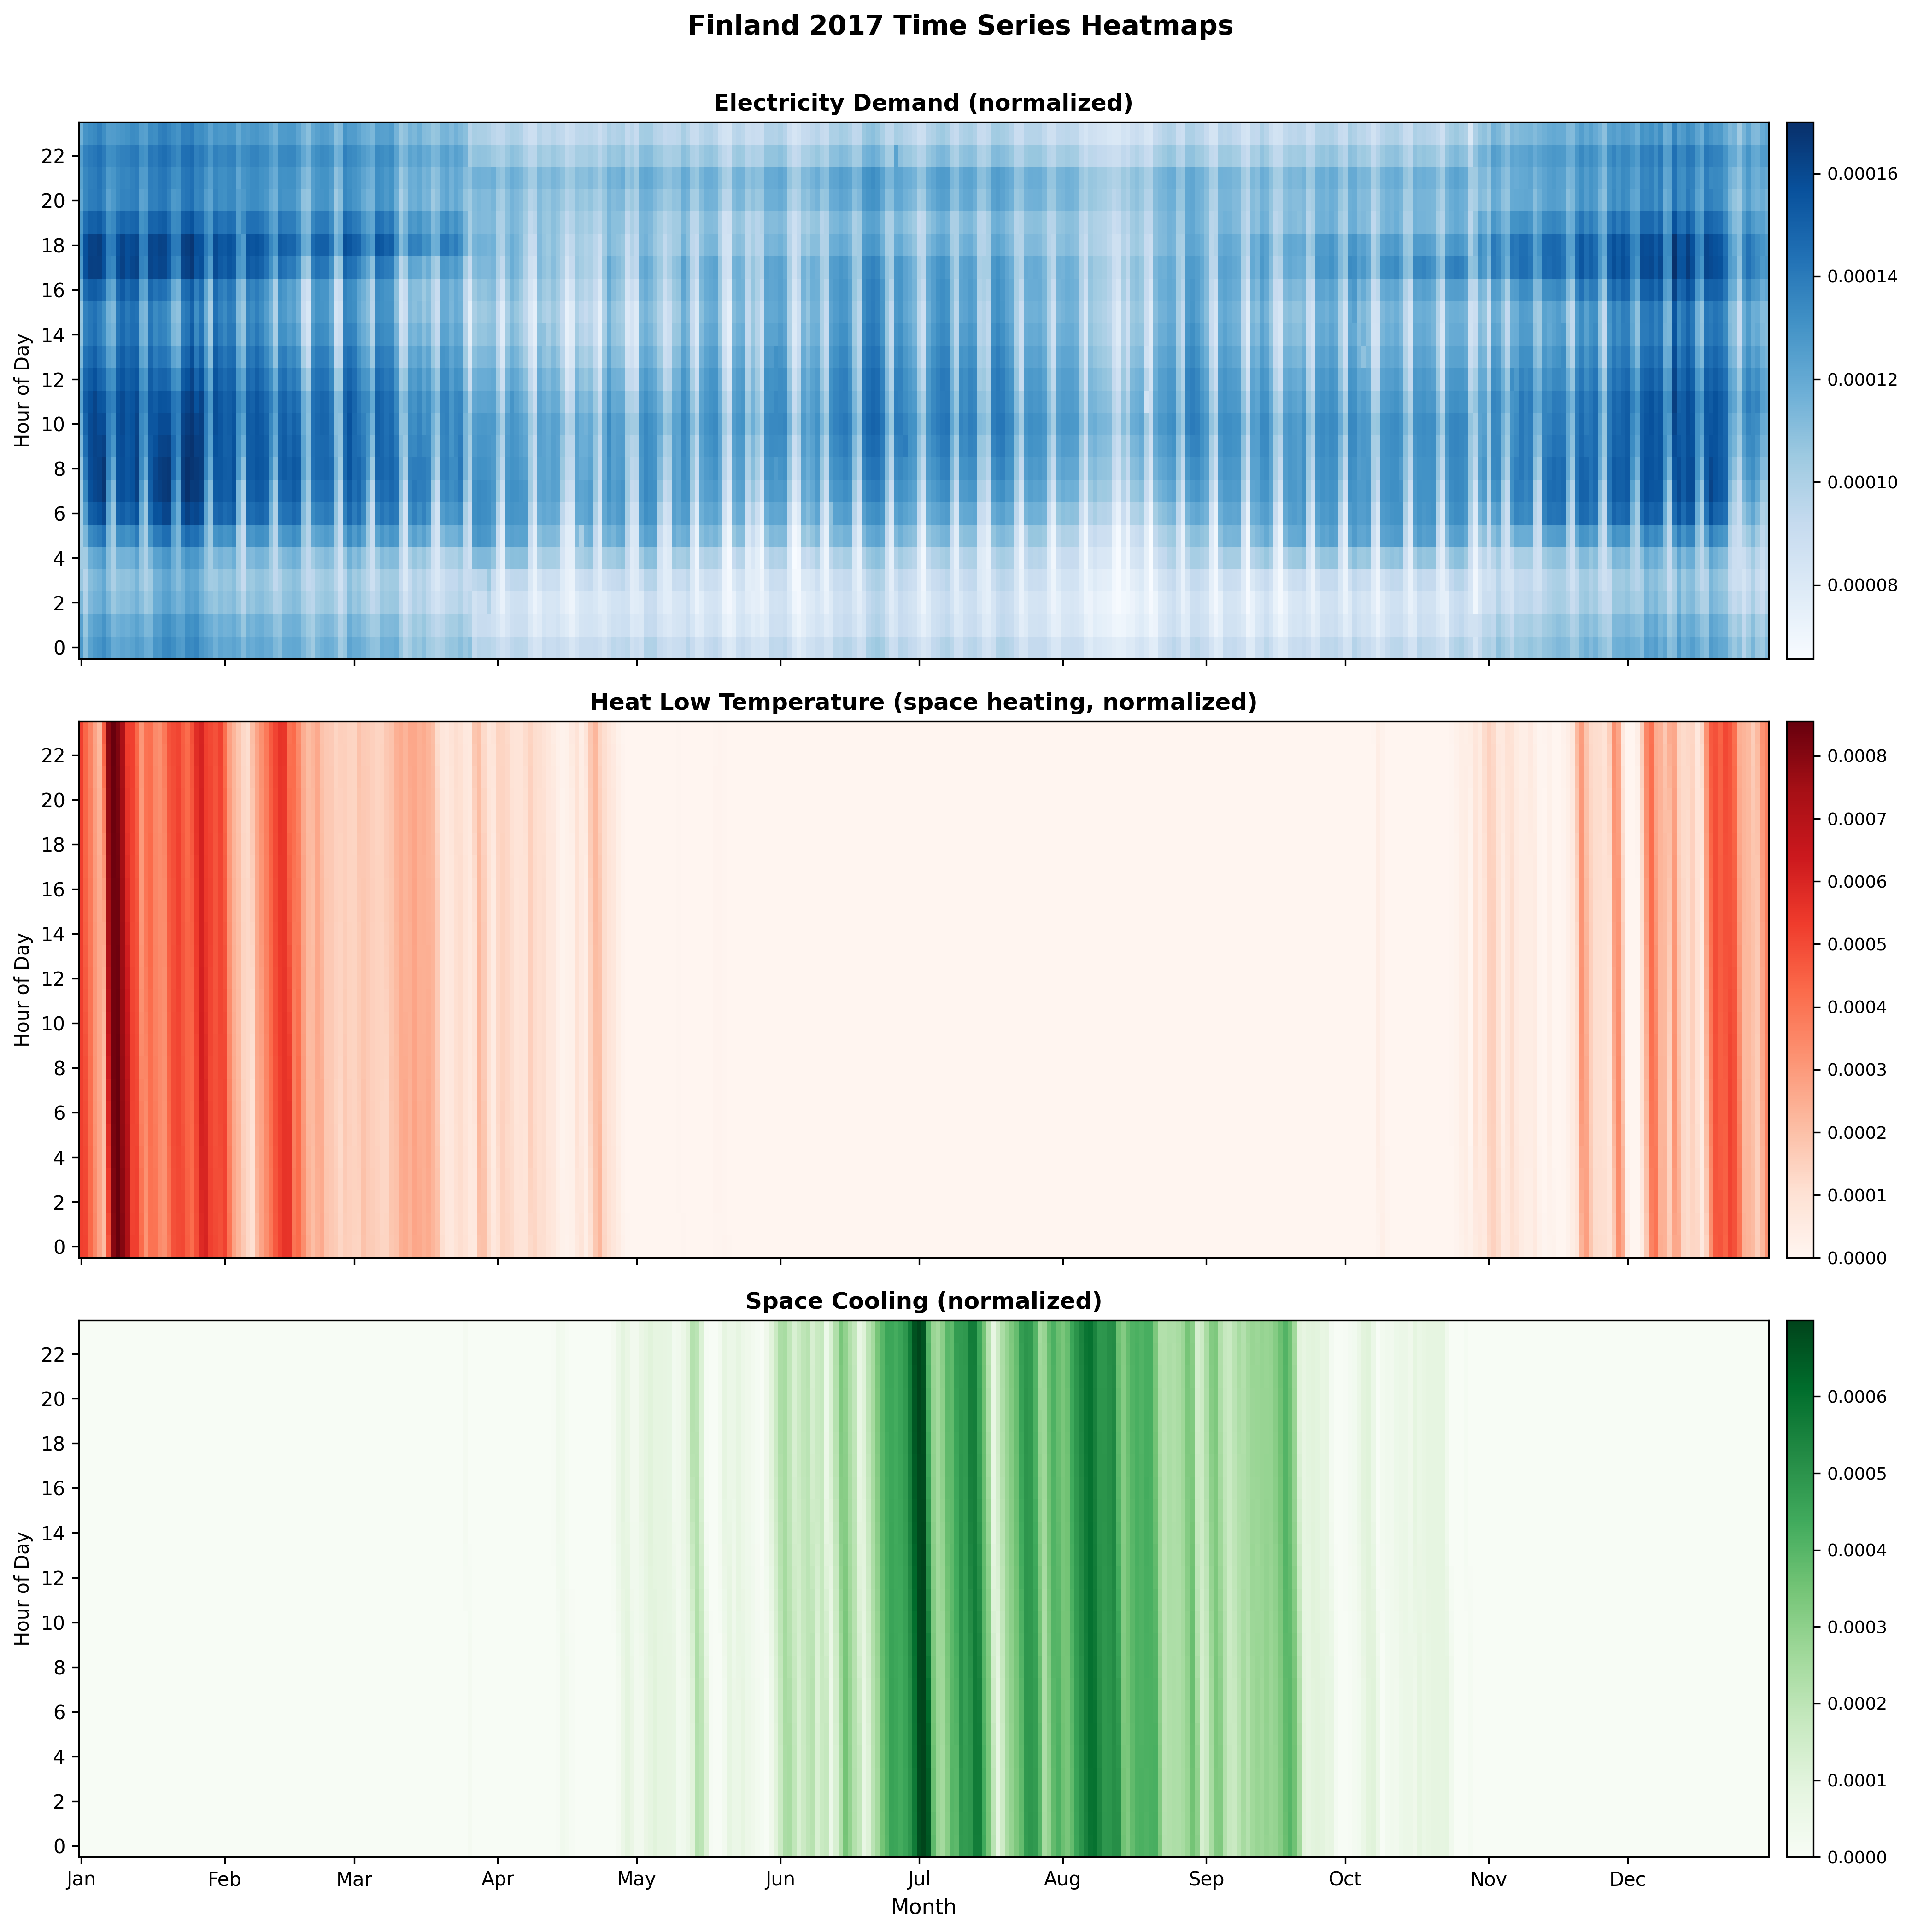
\includegraphics[width=\linewidth]{fi_heatmaps_combined.png}
  \caption{Finland (2017, UTC): demand-driver heatmaps used in the typical-day preprocessing. Each panel shows the distribution of hourly demand over the year (normalised profiles), with months on the x-axis and hour of day on the y-axis.}
  \label{fig:fi_td_demand_heatmaps}
\end{figure}

The electricity profile exhibits both intra-day structure (systematic daily cycles) and a marked seasonal component, with higher intensities during the cold season. Low-temperature space-heating demand is strongly seasonal, with a pronounced winter concentration and near-zero levels in summer, reflecting its degree-hour construction. Space-cooling appears as a sparse summer phenomenon, indicating that cooling is a minor driver in the Finnish context and contributes limited discriminatory information outside the warmest weeks. Because all demand series are normalised, the colour intensity should be read as the relative allocation of annual demand across hours rather than absolute load levels.


\begin{figure}[H]
  \centering
  
\includegraphics[width=0.78\linewidth]{FI_2017_mobility_passenger_daily_profile.png}
  \caption{Passenger mobility daily profile used in EnergyScope Multi-Cells (Finland application, 2017, UTC). The profile is adopted from the EnergyScope TD Belgium setup, itself based on a generic household travel survey hourly pattern, and repeated identically for each day of the year (time-zone mapped).}
  \label{fig:fi_td_mobility_daily}
\end{figure}

The passenger mobility profile is characterised by a morning ramp-up and a broad daytime plateau, followed by a steady decline in the evening. In this modelling framework, the curve is exogenous and does not vary across days, so it does not drive the identification of representative days in clustering. Its role is instead to provide within-day structure for mobility demand once typical days have been selected, ensuring consistent diurnal timing of transport services across scenarios.


\begin{figure}[H]
  \centering
  
\includegraphics[width=\linewidth]{FI_2017_heatmaps_main.png}
  \caption{Finland (2017, UTC): renewable availability heatmaps used as TD inputs. Panels report capacity-factor type hourly profiles for wind (onshore and offshore), solar (thermal proxy) and PV, plus hydropower proxies (dam inflow and run-of-river), and tidal (negligible for Finland, so not plotted)}
  \label{fig:fi_td_renewables_heatmaps}
\end{figure}

Solar and PV exhibit the expected joint diurnal and seasonal structure: near-zero availability during winter and night-time, with sustained daytime generation during summer months. Wind availability shows substantial hour-to-hour and day-to-day variability across the full year, providing strong discriminatory power for typical-day selection. Hydropower proxies are comparatively smoother, with changes that are more seasonal than diurnal, consistent with inflow-driven dynamics and the aggregation procedure used to derive normalised profiles. Together, these patterns motivate including multiple supply-side drivers in the clustering so that typical days reflect both short-term intermittency (wind) and seasonal solar scarcity.

\begin{figure}[H]
  \centering
  
\includegraphics[width=\linewidth]{fi_load_duration_curves.png}
  \caption{Finland (2017, UTC): load duration curves for normalised demand drivers. Curves show the ordered distribution of hourly values (descending), highlighting peakiness and the weight of extreme hours in annual demand profiles.}
  \label{fig:fi_td_duration_curves}
\end{figure}

The electricity duration curve is relatively smooth, indicating that a large portion of annual electricity demand is spread across many hours, with limited reliance on extreme peaks. By contrast, the low-temperature space-heating curve displays a steeper tail, consistent with winter-driven peaks that can materially affect capacity sizing and adequacy constraints. Passenger mobility exhibits a stepped structure because the same diurnal pattern is repeated throughout the year, while freight is flat in the compiled dataset and therefore appears as a constant line. These duration curves provide a compact diagnostic for the extent to which typical days must preserve peak and near-peak hours in order to reproduce sizing-relevant extremes.

As an additional diagnostic, Figure~\ref{fig:fi_td_daily_covariation} reports daily-mean co-variation between selected demand and renewable drivers. While typical-day clustering operates on 24-hour vectors rather than daily averages, these scatter plots clarify cross-variable seasonal structure and motivate retaining multiple drivers in the clustering space.

\begin{figure}[H]
  \centering
  
\includegraphics[width=\linewidth]{FI_2017_daily_mean_scatter.png}
  \caption{Finland (2017, UTC): daily-mean co-variation between selected TD drivers (colour indicates day of year). Demand variables are shown in per-mille of annual total per hour. Reported $r$ are Pearson correlations across daily means.}
  \label{fig:fi_td_daily_covariation}
\end{figure}


Heating and solar availability are strongly anti-correlated ($r=-0.693$), reflecting a seasonal mismatch in which high space-heating needs coincide with low solar resources. Electricity demand and PV availability display a weaker positive association ($r=0.330$), consistent with both being higher during brighter months while remaining dispersed due to day-to-day weather and non-climatic electricity drivers. Heating and onshore wind show near-independence ($r=0.175$), indicating that wind intermittency is largely orthogonal to heating seasonality; this supports retaining both heating and wind in the feature set so that typical days capture jointly stressful configurations (e.g., cold days with low wind).



In the typical-day construction, we prioritise the most informative drivers of hourly system constraints, namely electricity demand, low-temperature space-heating demand, space-cooling demand (when present), and the main weather-dependent renewable capacity factors (PV and wind, plus run-of-river hydro when available). By contrast, profiles that are flat or nearly invariant across days (for example freight demand in the compiled dataset) provide little discriminatory power for day selection and are therefore not used as primary clustering attributes.

\newpage

\subsubsection{Clustering and representative-day selection}
Let $x_{k,d,h}$ denote the value of time series $k$ at hour $h$ of day $d$. A clustering procedure partitions the $D=365$ days into $N$ clusters, each represented by one TD. In the EnergyScope TD literature, several clustering and representative-day selection strategies are compared, including k-medoids and alternative heuristics; their relative performance depends on the trade-off between computational effort and approximation accuracy \citep{Limpens2021Thesis,thiranExploringOptionsFossilfree2025}. The output of this stage is:
(i) a set of TDs,
(ii) a mapping $td(d)$ assigning each original day to a TD, and
(iii) weights $w_{td}$ (the number of original days represented by each TD).

\subsubsection{Chronological reconstruction and storage coupling}
A limitation of TD-based representations is that they can break chronology, which is problematic for storage technologies whose optimal operation depends on sequences of days rather than isolated daily shapes. EnergyScope TD addresses this issue by coupling TD operation with a chronological reconstruction of the year, so that storage state variables evolve over the full horizon while most operational decisions remain defined on the reduced TD set \citep{dominguez-munoz_selection_2011,limpensEnergyScopeTDNovel2019}.

The underlying idea can be understood over a one-week sequence. Calendar days are represented as an ordered list of TD labels (for example, TD~1 on Monday, TD~2 on Tuesday and Wednesday, and TD~3 on weekend days). For a given TD, the intra-day charging and discharging power profile is repeated whenever that TD appears in the sequence, but the stored-energy level is not repeated day by day. Instead, the state of charge is tracked continuously across the entire chronology, linking the end-of-day storage level to the start of the next day even when successive days correspond to different TDs. In practice, this coupling allows the model to exploit TDs to capture typical within-day patterns while still representing inter-day and seasonal storage strategies, such as progressively building reserves across sequences of surplus days and drawing them down during extended deficit periods.

\subsubsection{Optimising the TD set: error metrics and MILP formulation}
EnergyScope TD formalises TD selection using an optimisation-based procedure (MILP) that aims to reduce the approximation error of the reduced time representation. Two complementary error notions are commonly used:
\begin{itemize}
  \item \textbf{Clustering (chronological-shape) error}, measuring how well each day is represented hour-by-hour by its assigned TD.
  \item \textbf{Duration-curve error}, measuring how well the reduced representation reproduces the sorted distribution of hourly values (important for peaks and scarcity periods).
\end{itemize}
A generic formulation (notation adapted from \citet{limpensEnergyScopeTDNovel2019}) is:
\begin{align}
E_{\mathrm{clust}} &= \sum_{k \in \mathcal{K}} \alpha_k \sum_{d=1}^{D} \sum_{h=1}^{24} \left(x_{k,d,h} - \tilde{x}_{k,td(d),h}\right)^2, \\
E_{\mathrm{dc}} &= \sum_{k \in \mathcal{K}} \beta_k \sum_{t=1}^{8760} \left(\mathrm{DC}_k(t) - \widetilde{\mathrm{DC}}_k(t)\right)^2,
\end{align}
where $\mathrm{DC}_k(\cdot)$ is the duration curve (sorted hourly values) of series $k$, and tildes denote the reconstructed values from the TD representation. The MILP chooses the TD set (and assignments) to minimise a weighted combination of these errors subject to selecting exactly $N$ representative days.

Previous EnergyScope TD applications commonly rely on $12$ typical days, which has been identified as a robust compromise between temporal accuracy and computational tractability. In the original EnergyScope TD validation, moving from a full 8{,}760-hour representation to 12 TDs reduces solve times from multi-hour runs to around a minute, making large scenario ensembles and sensitivity analyses feasible. At the same time, 12 TDs were shown to reproduce the full-year ``ground-truth'' solution reasonably well for the main key performance indicators used in planning exercises, including primary energy use, technology capacity choices, total system cost, and aggregate greenhouse-gas emissions. Consistent with this established practice, the present Finland application adopts 12 typical days as a baseline; alternative values can be explored later as a robustness check once the dataset calibration and historical reproduction are consolidated.


\subsection{Step 2: EnergyScope TD optimisation model}

\subsubsection{LP problem: resources, layers, and technologies}
EnergyScope TD represents the energy system as a network of energy \emph{layers} that must be balanced at each time step. Layers include both resources (e.g. natural gas, biomass, solar) and end-use demand layers (e.g. low-temperature heat, passenger mobility), and technologies connect layers through conversion, storage, or infrastructure. Following the EnergyScope terminology, three technology types are distinguished:
(i) end-use type technologies (producing end-use demand layers),
(ii) storage technologies (inter-temporal links within a layer),
and (iii) infrastructure technologies (supporting conversion, networks, and efficiency).

EnergyScope TD is formulated as an LP problem in which the main design variables are installed capacities $F(j)$ for technologies $j$, and the main operational variables are hourly flows (resource uses and technology outputs) defined over hours $h$ and TDs $td$ \citep{limpensGeneratingEnergyTransition2021}. This structure enables rapid solution times that are compatible with extensive scenario sampling. 


The LP solved by EnergyScope TD can be read as a network of balance equations and flow constraints: each coloured \emph{layer} corresponds to an energy-balance equation enforced at every hour (and for each typical day), while each connection corresponds to a non-negative flow variable constrained by technology capacities and conversion coefficients. The solver jointly chooses (i) \emph{design} variables, the installed sizes of assets, and (ii) \emph{operation} variables, the hourly routing of energy through competing pathways to meet end-use demands at minimum system cost. In this network view, storage technologies add inter-temporal coupling by shifting flows across hours, while infrastructure introduces losses and capacity limits, so that the optimum emerges from trading off direct supply, conversion, storage, and cross-sector coupling under resource availability and demand constraints.



\subsubsection{End-use demand in energy services (EUD)}
Following \citet{moretStrategicEnergyPlanning2017}, EnergyScope specifies exogenous \emph{end-use demand} (EUD) in terms of energy services rather than \emph{final energy consumption} (FEC). EUD refers to the useful service delivered to end users (e.g., low-temperature heat, passenger-kilometres, ton-kilometres), whereas FEC depends on the chosen conversion pathway and its efficiency. Model inputs are annual sectoral EUD values $endUsesYear(eui,s)$, aggregated into a yearly vector $endUsesInput(eui)$. These yearly totals are then allocated to period-specific demands $EndUses(eut,t)$ through transparent distribution and split rules (Fig.~\ref{fig:enduses_flow}): electricity is distributed uniformly over periods and corrected for grid losses $Loss(Elec,t)$; high-temperature heat is also spread uniformly; low-temperature heat combines space-heating, shaped by an exogenous profile $\%_{\mathrm{sh}}(t)$, with hot-water demand, then splits into district heating and decentralised supply using $\%_{\mathrm{Dhn}}$ (including DHN losses $Loss(HeatLowTDhn,t)$); finally, passenger and freight mobility are distributed uniformly and partitioned by modal shares $\%_{\mathrm{Public}}$ and $\%_{\mathrm{Rail}}$. Consistent with the mapping in Fig.~\ref{fig:enduses_flow}, lighting is not represented as a separate end-use and is instead included in the aggregate electricity end-use. The allocation and split parameters (e.g., $\%_{\mathrm{Public}}$, $\%_{\mathrm{Rail}}$, $\%_{\mathrm{Dhn}}$, and the space-heating profile $\%_{\mathrm{sh}}(t)$) are country-specific, as they reflect national patterns in modal shares, heating infrastructures, and seasonal demand. In the Finnish application, these parameters therefore need to be calibrated to Finland using national energy and transport statistics to ensure that the mapping from $endUsesInput$ to $EndUses(eut,t)$ matches observed end-use structures (see Table \ref{tab:fin_eud_params_2020}).


The monthly totals obtained by summing the compiled hourly profiles provide a simple diagnostic of how yearly end-use demand is allocated across the calendar. Because each series is normalised over the year, monthly sums should be read as shares of the annual end-use rather than as absolute energy levels. In the Finnish case, this diagnostic confirms the strong winter concentration of low-temperature space-heating demand, whereas electricity remains comparatively flatter across months and passenger mobility remains close to uniform because its diurnal shape is repeated throughout the year in the compiled dataset. This seasonality check helps identify which end-uses provide the strongest temporal signal that the typical-day selection must preserve.



\begin{figure}[t]
\centering
\resizebox{0.98\linewidth}{!}{%
\begin{tikzpicture}[
  font=\small,
  flow/.style={line width=0.6pt, line cap=round},
  lblL/.style={anchor=east, align=left},
  lblR/.style={anchor=west, align=left},
  lab/.style={font=\scriptsize, inner sep=1pt, fill=white},
  sum/.style={circle, draw, line width=0.6pt, inner sep=1.3pt}
]

\def\xLabelL{0.0}
\def\xStart{1.2}
\def\xJoin{8.0}
\def\xSplit{10.2}
\def\xEnd{15.2}
\def\xLabelR{16.1}

\def\yElec{5.0}
\def\yHT{3.9}
\def\ySH{2.6}
\def\yHW{1.7}
\def\yPass{0.4}
\def\yFre{-0.7}

\def\yDHN{2.9}
\def\yDec{2.1}
\def\yPub{0.8}
\def\yPriv{0.0}
\def\yRail{-0.4}
\def\yRoad{-1.2}

% ------------------------
% Headings (fixed, no overlap)
% ------------------------
\node[anchor=south west] at (\xStart,\yElec+1.05)
{$endUsesInput(eui)=\sum_{s\in S} endUsesYear(eui,s)\qquad \forall eui\in EUI$};

\node[anchor=south east] at (\xEnd,\yElec+1.05)
{$EndUses(eut,t)$};

% Left labels
\node[lblL] at (\xLabelL,\yElec) {ELECTRICITY};
\node[lblL] at (\xLabelL,\yHT)   {HEAT HIGH T};
\node[lblL] at (\xLabelL,\ySH)   {HEAT LOW T (SH)};
\node[lblL] at (\xLabelL,\yHW)   {HEAT LOW T (HW)};
\node[lblL] at (\xLabelL,\yPass) {MOB.\ PASSENGER};
\node[lblL] at (\xLabelL,\yFre)  {MOB.\ FREIGHT};

% Right labels
\node[lblR] at (\xLabelR,\yElec) {ELECTRICITY};
\node[lblR] at (\xLabelR,\yHT)   {HEAT HIGH T};
\node[lblR] at (\xLabelR,\yDHN)  {HEAT LOW T DHN};
\node[lblR] at (\xLabelR,\yDec)  {HEAT LOW T DECEN};
\node[lblR] at (\xLabelR,\yPub)  {MOB.\ PUBLIC};
\node[lblR] at (\xLabelR,\yPriv) {MOB.\ PRIVATE};
\node[lblR] at (\xLabelR,\yRail) {MOB.\ FREIGHT RAIL};
\node[lblR] at (\xLabelR,\yRoad) {MOB.\ FREIGHT ROAD};

% Electricity (lighting omitted)
\draw[flow] (\xStart,\yElec) -- (\xEnd,\yElec)
  node[lab, pos=0.46, above=2pt] {$\cdot \dfrac{1}{\sum_{t'\in T} t_{op}(t')}$}
  node[lab, pos=0.74, above=2pt] {$+\,Loss(Elec,t)$};

% Heat high T
\draw[flow] (\xStart,\yHT) -- (\xEnd,\yHT)
  node[lab, pos=0.46, above=2pt] {$\cdot \dfrac{1}{\sum_{t'\in T} t_{op}(t')}$};

% Low-T heat: SH + HW then split
\node[sum] (sumHeat) at (\xJoin,2.15) {$+$};

\draw[flow] (\xStart,\ySH) -- (\xJoin-1.6,\ySH)
  node[lab, pos=0.55, above=2pt] {$\cdot \dfrac{\%_{\mathrm{sh}}(t)}{t_{op}(t)}$}
  -- (\xJoin-1.6,2.15) -- (sumHeat.west);

\draw[flow] (\xStart,\yHW) -- (\xJoin-1.6,\yHW)
  node[lab, pos=0.55, below=2pt] {$\cdot \dfrac{1}{\sum_{t'\in T} t_{op}(t')}$}
  -- (\xJoin-1.6,2.15) -- (sumHeat.west);

\coordinate (heatSplit) at (\xSplit,2.15);
\draw[flow] (sumHeat.east) -- (heatSplit);

\draw[flow] (heatSplit) -- (\xEnd,\yDHN)
  node[lab, pos=0.56, above=2pt] {$\cdot \%_{\mathrm{Dhn}} \;+\; Loss(HeatLowTDhn,t)$};

\draw[flow] (heatSplit) -- (\xEnd,\yDec)
  node[lab, pos=0.56, below=2pt] {$\cdot (1-\%_{\mathrm{Dhn}})$};

% Passenger mobility split
\coordinate (passSplit) at (\xSplit,\yPass);
\draw[flow] (\xStart,\yPass) -- (passSplit)
  node[lab, pos=0.52, above=2pt] {$\cdot \dfrac{1}{\sum_{t'\in T} t_{op}(t')}$};

\draw[flow] (passSplit) -- (\xEnd,\yPub)
  node[lab, pos=0.56, above=2pt] {$\cdot \%_{\mathrm{Public}}$};

\draw[flow] (passSplit) -- (\xEnd,\yPriv)
  node[lab, pos=0.56, below=2pt] {$\cdot (1-\%_{\mathrm{Public}})$};

% Freight mobility split
\coordinate (freSplit) at (\xSplit,\yFre);
\draw[flow] (\xStart,\yFre) -- (freSplit)
  node[lab, pos=0.52, above=2pt] {$\cdot \dfrac{1}{\sum_{t'\in T} t_{op}(t')}$};

\draw[flow] (freSplit) -- (\xEnd,\yRail)
  node[lab, pos=0.56, above=2pt] {$\cdot \%_{\mathrm{Rail}}$};

\draw[flow] (freSplit) -- (\xEnd,\yRoad)
  node[lab, pos=0.56, below=2pt] {$\cdot (1-\%_{\mathrm{Rail}})$};

\end{tikzpicture}%
}
\caption{Mapping from yearly end-use inputs $endUsesInput$ to period-specific demands $EndUses(eut,t)$, with lighting aggregated into the electricity end-use. Adapted from \citet{moret_strategic_2017}.}
\label{fig:enduses_flow}
\end{figure}

\begin{table}[h!]
\footnotesize
\centering
\begin{threeparttable}
\caption{Finland calibration targets for the EUD mapping (baseline year 2020).}
\label{tab:fin_eud_params_2020}

% Choose a width for the Source column that fits your page.
% Here: last column wraps at ~55% of linewidth.
\begin{tabular}{@{} l l l >{\raggedright\arraybackslash}p{0.35\linewidth} @{}}
\toprule
Parameter & Symbol & Value & Source \\
\midrule
District heating share of low-T heat\tnote{a} &
$\%_{\mathrm{Dhn}}$ &
0.45 &
\href{https://energia.fi/wp-content/uploads/2024/01/Energy-Year-2023_DistrictHeating.pdf}{Finnish Energy (2024)} \\

District heating network losses\tnote{b} &
$Loss(\mathrm{HeatLowTDhn})$ &
0.085 &
\href{https://energia.fi/en/energy-sector-in-finland/energy-networks/district-heating-networks/}{Finnish Energy (2024)} \\

Inland public passenger mobility share\tnote{c} &
$\%_{\mathrm{Public}}$ &
0.1608 &
\href{https://stat.fi/til/tiet/2019/tiet_2019_2020-04-15_en.pdf}{Statistics Finland (2020), \emph{Traffic on highways 2019}}
; \href{https://stat.fi/til/rtie/2019/rtie_2019_2020-08-27_en.pdf}{Statistics Finland (2020), \emph{Railway statistics 2019}} \\

Inland rail freight share\tnote{d} &
$\%_{\mathrm{Rail}}$ &
0.2761 &
\href{https://stat.fi/til/rtie/2019/rtie_2019_2020-08-27_en.pdf}{Statistics Finland (2020), \emph{Railway statistics 2019}}
; \href{https://stat.fi/til/kttav/2019/kttav_2019_2020-04-28_en.pdf}{Statistics Finland (2020), \emph{Goods transport by road 2019}} \\

Electricity grid losses\tnote{e} &
$Loss(\mathrm{Elec})$ &
0.03 &
\href{https://www.doria.fi/bitstream/10024/185778/1/yene_efp_202200_2022_25869_net.pdf}{Finnish Energy and Statistics Finland (2022), \emph{Energy in Finland 2022}} \\
\bottomrule
\end{tabular}

\begin{tablenotes}\footnotesize
\item[a] Proxy for the DHN split: district heating share of heating energy / space-heating market in Finland (year 2020).
\item[b] Implemented as a constant loss factor; Finnish Energy reports typical DH distribution losses of 8--9\% of transmitted energy, hence 0.085 as midpoint.
\item[c] Computed as $(\mathrm{pkm}_{\mathrm{bus}}+\mathrm{pkm}_{\mathrm{rail}})/(\mathrm{pkm}_{\mathrm{car}}+\mathrm{pkm}_{\mathrm{bus}}+\mathrm{pkm}_{\mathrm{rail}})$ using pre-COVID 2019 inland passenger-km: $\mathrm{pkm}_{\mathrm{car}}=66.8$ bn and $\mathrm{pkm}_{\mathrm{bus}}=7.9$ bn (\emph{Traffic on highways 2019}), and $\mathrm{pkm}_{\mathrm{rail}}=4.9$ bn (\emph{Railway statistics 2019}). 2019 is used as a structural proxy to avoid pandemic-related distortions in 2020 modal shares.
\item[d] Computed as $\mathrm{tkm}_{\mathrm{rail}}/(\mathrm{tkm}_{\mathrm{rail}}+\mathrm{tkm}_{\mathrm{road}})$ using pre-COVID 2019 inland freight tonne-km: $\mathrm{tkm}_{\mathrm{rail}}=10.3$ bn (\emph{Railway statistics 2019}) and $\mathrm{tkm}_{\mathrm{road}}\approx 27.0$ bn from domestic road freight performance reported as ``close on 27 million tonne-kilometres'' in \emph{Goods transport by road 2019} (interpreted as 27,000 million tonne-km).
\item[e] Electricity transmission and distribution losses are set to 0.03 based on the ``Losses 3\%'' entry reported in the electricity consumption breakdown in \emph{Energy in Finland 2022} (compiled from Finnish Energy and Statistics Finland). Used as a constant proxy for baseline year 2020.
\end{tablenotes}
\end{threeparttable}
\end{table}





\subsubsection{Objective function: total annual cost (and emissions accounting)}
A standard objective is the minimisation of total annualised system cost,
decomposed into annualised investment costs, fixed operation and maintenance costs, and resource operating costs \citep{limpensEnergyScopeTDNovel2019}:
\begin{align}
\min \; C_{\mathrm{tot}}
= \sum_{j \in \mathcal{TECH}} \left[\tau(j)\, C_{\mathrm{inv}}(j) + C_{\mathrm{maint}}(j)\right]
+ \sum_{i \in \mathcal{RES}} C_{\mathrm{op}}(i),
\end{align}
with $\tau(j)$ an annualisation factor that depends on the discount rate and lifetime. 
In addition, annual system-wide GHG emissions are computed with a life cycle assessment approach, accounting for “cradle-to-grave” emissions from both technologies and energy resources. Climate impacts are reported using global warming potential (GWP) in ktCO\textsubscript{2}-eq per year. Total yearly emissions, $GWP_{\text{tot}}$ (Eq.~\eqref{eq:gwp_total}), are defined as the sum of (i) the construction and end-of-life impacts of energy conversion technologies, annualised by their lifetime, and (ii) operational impacts from resources, including fuel supply chains (up to combustion) and imported electricity, weighted by the operating period.

Following \citet{limpensEnergyScopeTDNovel2019}:

\begin{equation}
GWP_{\mathrm{tot}} \;=\; \sum_{j \in \mathrm{TECH}} \frac{GWP_{\mathrm{constr}}(j)}{\mathrm{lifetime}(j)} \;+\; \sum_{i \in \mathrm{RES}} GWP_{\mathrm{op}}(i)
\label{eq:gwp_total}
\end{equation}
 


\subsubsection{Seasonality and long-term storage: coupling typical days}
A known limitation of TD approaches is the difficulty to represent inter-day dynamics and seasonal storage. EnergyScope TD implements a reconstruction method in which each day of the year is assigned to a TD through a sequence, while the stored-energy state variable is tracked across all 8760 hours. Operational variables other than stored energy remain defined on the TD basis \citep{limpensGeneratingEnergyTransition2021}. This enables modelling of day-to-day and seasonal storage strategies without solving the full hourly year.

Because EnergyScope TD is designed for fast whole-system optimisation, it abstracts from some short-term operational details (e.g. unit commitment or detailed ramping constraints) that are central in dispatch-focused models. The TD approach is therefore best interpreted as a planning-level representation that trades operational detail for tractability, and can be complemented by more detailed operational checks when needed \citep{thiranExploringOptionsFossilfree2025}.


% ------------------------------------------------------------------
\subsubsection{Biomass modelling: feedstocks, supply curves, and Finland-specific calibration}
\label{sec:biomass_modelling}

Bioenergy potentials are not uniquely defined objects: reported values differ widely because they embed distinct assumptions about sustainability constraints, competing uses (materials, soil functions, circularity), land allocation for energy crops, and waste management pathways. Selecting a given ``potential'' is therefore a structural modelling choice that shapes the socio-technical system being represented. \citet{collaNavigatingBioenergyHorizons2024} illustrate this point by showing that European assessments can imply markedly different 2030 bioenergy ranges for a single country (Belgium: 30--90~TWh across four studies), with divergences driven primarily by (i) how competing uses are accounted for, (ii) land-use rules for energy crops, and (iii) whether waste streams are directed to energy or material recovery. At the European scale, they argue that a ``realistic'' order of magnitude for EU27+UK in 2030 lies in the lower part of published ranges (about 2000--2500~TWh), noting that forestry feedstocks are already relatively exploited while additional mobilisation would come mainly from agricultural residues, conditional on collection practices and farm structure \citep{collaNavigatingBioenergyHorizons2024}. These lessons motivate a transparent, scenario-based calibration strategy for Finland rather than reliance on a single headline potential.

The Belgian application of \citet{collaOptimalUseLignocellulosic2022} presents lignocellulosic biomass through cost supply curves, an origin-by-quality decomposition, and step-specific embedded GHG intensities. Their Belgium case therefore makes three modelling choices explicit: biomass is procured in merit order, different fractions have different marginal costs, and different fractions carry different supply-chain carbon footprints. We retain that logic in the Finnish first stage because it is the right level of detail for asking where a scarce biomass resource is most valuable once system-wide GHG constraints bind.

The current Finnish implementation does not reproduce the full Belgian origin-by-quality matrix. Instead, it collapses the forest-biomass ladder into four domestic steps and one import backstop. This is a deliberate simplification because the present paper studies forest-management intensity and biodiversity constraints in Finland, not the full geography of European biomass trade. Four simplifications should therefore be stated explicitly:
\begin{enumerate}
  \item The domestic ladder aggregates the Finnish forest resource into industrial by-products, logging residues, secondary woodchips/sawdust, and direct fuelwood/landscape wood, rather than distinguishing all Belgian origin rings and quality classes separately.
   \item Step-specific embedded GHG coefficients are assigned by matching each Finnish step to the most appropriate EU RED~II Annex~VI supply-chain category as tabulated by \citet{collaOptimalUseLignocellulosic2022} (see Table~\ref{tab:fi_biomass_ladder} caption for the per-step mapping). The GHG merit order is not monotone with the cost merit order: mill-gate and industrial wood residues (FI1, FI3) have shorter supply chains than in-forest collected logging residues (FI2), so FI3 carries lower supply-chain GHG (14~tCO$_2$eq/GWh) than FI2 (22~tCO$_2$eq/GWh) despite being more costly. Finnish-specific LCA validation would be needed to confirm these values rigorously.
 
  \item The Belgian low-quality share constraint is not re-implemented at this stage. The Finnish first-stage model therefore captures relative cost and relative GHG differences between steps, but not a separate ash-content or quality-mixing constraint.
  \item The Finnish scenarios are parameterised to represent forest-policy narratives, not to claim direct measurement of future biomass availability. In particular, S1/BES is stylised and S3/BDS is a conservative audited scenario rather than a raw database value.
\end{enumerate}

Let $r \in \{\text{WOOD\_FI1},\dots,\text{WOOD\_FI5}\}$ denote a Finnish biomass step. We introduce decision variables $x_r$ (annual energy procured from step $r$), with exogenous step capacities $\overline{X}_r$, marginal supply costs $c_r$, and embedded supply-chain GHG intensities $g_r$. The first-stage formulation is:
\begin{align}
0 \leq x_r &\leq \overline{X}_r \qquad \forall r,
\label{eq:bio_segment_cap}\\
C_{\text{bio}} &= \sum_r c_r\,x_r,
\label{eq:bio_cost}\\
\text{GHG}_{\text{bio,supply}} &= \sum_r g_r\,x_r.
\label{eq:bio_ghg}
\end{align}
The optimiser first uses the cheapest domestic fractions and only reaches the high-cost import backstop when cheaper Finnish steps are exhausted.

The neutral reference case S2/NFS is built from the ENSPRESO medium potential for Finland, interpolated to 2035 at the commodity-code level before aggregation into the four domestic steps \citep{ruizENSPRESOOpenEU282019}. The stylised S1/BES case is then constructed as a +20\% scale-up of the S2 ladder. This is not presented as a literal replication of the BES harvest simulated by \cite{blattertSectoralPoliciesCause2022}; it is a sensitivity case used because the ENSPRESO high scenario for Finland yields implausibly large forest-energy volumes and because the BES narrative increases some residue streams without simply increasing all wood categories proportionally. Importantly, \citet{blattertSectoralPoliciesCause2022} find that under its biodiversity non-decline constraint BES achieves only 75\% of the maximum possible harvest, with the harvest mix shifting toward more logging biomass and less roundwood relative to NFS. The +20\% parameterisation is therefore a deliberate upper-bound sensitivity that follows the BES direction of intensified biomass mobilisation without claiming to replicate the Blattert BES harvest volumes quantitatively. The conservative S3/BDS case is not the original ENSPRESO low value of 74.2~TWh. That initial value was revised downward after a three-way audit combining the biodiversity-constrained forest-management narrative of Blattert et al., the ecological harvest ceiling proposed by M\"onkk\"onen et al., and a cross-check against recent Finnish national wood-energy statistics \citep{blattertSectoralPoliciesCause2022,monkkonenEcologicallyEconomicallySustainable2024,lukeWoodEnergy2024}. The revised domestic S3 ceiling is 40~TWh, split across the four domestic steps as 32.0, 6.0, 1.5, and 0.5~TWh. The logging-residue step (\texttt{WOOD\_FI2}) also carries a 4~€/MWh cost premium under S3/BDS (26 versus 22~€/MWh in S1/S2). This reflects two BDS-specific cost drivers: lower per-hectare residue yields because the biodiversity strategy requires retaining a fraction of coarse woody debris as deadwood on site \citep{blattertSectoralPoliciesCause2022,monkkonenEcologicallyEconomicallySustainable2025}, and longer average extraction distances because conservation set-asides restrict the accessible harvesting area. The resulting premium of $\approx$18\% above the S2 base cost is an explicit modelling assumption in the absence of published Finnish per-unit extraction costs for BDS-compliant harvesting; it is flagged as a parametric sensitivity.


\begin{table}[H]
\centering
\footnotesize
\caption{First-stage Finnish forest-biomass ladder used in the 2035 scenarios. Embedded GHG covers supply-chain only (harvesting, preprocessing, transport); biogenic combustion CO$_2$ is excluded. GHG values are assigned per step from EU RED~II Annex~VI supply-chain defaults as tabulated by \citet{collaOptimalUseLignocellulosic2022}: \textbf{FI2} (logging residues) uses the local forest-residue value (case~3a, $\leq$500~km, 21.6~tCO$_2$eq/GWh $\approx$~22); \textbf{FI3} (secondary mill residues) uses the agricultural/short-supply-chain proxy (case~7a, 14.4~tCO$_2$eq/GWh $\approx$~14) as a conservative upper bound for processing-site residues; \textbf{FI4} (fuelwood $+$ landscape-care wood) blends the fuelwood component (case~3a, $\approx$22) and the landscape-care component (case~7a, $\approx$14) at an approximate 60/40 ratio, giving $\approx$19~tCO$_2$eq/GWh; \textbf{FI1} (mill-gate by-products) is set at approximately half the forest-residue baseline (10~tCO$_2$eq/GWh), reflecting the absent in-forest collection and forwarding steps; \textbf{FI5} (rest-of-world backstop) uses the long-haul proxy (case~3a, $>$10{,}000~km, 39.6~tCO$_2$eq/GWh $\approx$~40). These RED~II-derived values are implemented in the model input files used for all scenario runs reported in this paper.}
\label{tab:fi_biomass_ladder}
\begin{tabularx}{\linewidth}{>{\raggedright\arraybackslash}p{2.2cm}X>{\centering\arraybackslash}p{2.2cm}>{\centering\arraybackslash}p{2.3cm}}
\toprule
\textbf{Step} & \textbf{Interpretation and main source mapping} & \textbf{Cost} & \textbf{Embedded GHG} \\
 &  & \textbf{(€/MWh)} & \textbf{(tCO$_2$eq/GWh)} \\
\midrule
\texttt{WOOD\_FI1} & Industrial by-products from chemical and physical wood processing, primarily black liquor, bark, and sawdust (ENSPRESO \texttt{MINBIOWOOa}) & 11 & 10 \\
\texttt{WOOD\_FI2} & Logging residues such as branches and tops (ENSPRESO \texttt{MINBIOFRSR1}) & 22 in S1/S2; 26 in S3 & 22 \\
\texttt{WOOD\_FI3} & Secondary woodchips and sawdust streams (ENSPRESO \texttt{MINBIOWOOW1} + \texttt{MINBIOWOOW1a}) & 27 & 14 \\
\texttt{WOOD\_FI4} & Direct fuelwood and landscape-care wood (ENSPRESO \texttt{MINBIOWOO} + \texttt{MINBIOFRSR1a}) & 33 & 19 \\
\texttt{WOOD\_FI5} & Rest-of-world biomass import backstop; GHG follows the Colla rest-of-world proxy (39.6 rounded to 40~tCO$_2$eq/GWh) & 70 & 40 \\
\bottomrule
\end{tabularx}
\end{table}

\begin{table}[H]
\centering
\footnotesize
\caption{Step capacities (TWh/yr) in the three 2035 forest-management scenarios. S2/NFS values are derived from ENSPRESO medium potentials interpolated to 2035 \citep{ruizENSPRESOOpenEU282019}; S1/BES applies a uniform $+20\%$ scale-up to all four S2 domestic steps; S3/BDS capacities are revised from the ENSPRESO low value following a three-way biodiversity-ceiling audit \citep{blattertSectoralPoliciesCause2022,monkkonenEcologicallyEconomicallySustainable2024,lukeWoodEnergy2024}. Step costs are given in Table~\ref{tab:fi_biomass_ladder}.}
\label{tab:fi_biomass_capacities}
\begin{tabularx}{\linewidth}{>{\raggedright\arraybackslash}p{2.2cm}X>{\centering\arraybackslash}p{1.65cm}>{\centering\arraybackslash}p{1.65cm}>{\centering\arraybackslash}p{1.65cm}}
\toprule
\textbf{Step} & \textbf{Main feedstock} & \textbf{S1-BES (TWh)} & \textbf{S2-NFS (TWh)} & \textbf{S3-BDS (TWh)} \\
\midrule
\texttt{WOOD\_FI1} & Industrial by-products (black liquor, bark, sawdust) & 54.5 & 45.4 & 32.0 \\
\texttt{WOOD\_FI2} & Logging residues (branches, tops) & 45.9 & 38.2 & 6.0 \\
\texttt{WOOD\_FI3} & Secondary woodchips and sawdust & 15.1 & 12.5 & 1.5 \\
\texttt{WOOD\_FI4} & Fuelwood and landscape-care wood & 6.5 & 5.4 & 0.5 \\
\texttt{WOOD\_FI5} & Baltic/Nordic import backstop & \multicolumn{3}{c}{unlimited} \\
\midrule
\textbf{Domestic total} & & \textbf{122.0} & \textbf{101.5} & \textbf{40.0} \\
\bottomrule
\end{tabularx}
\end{table}

\begin{figure}[H]
  \centering
  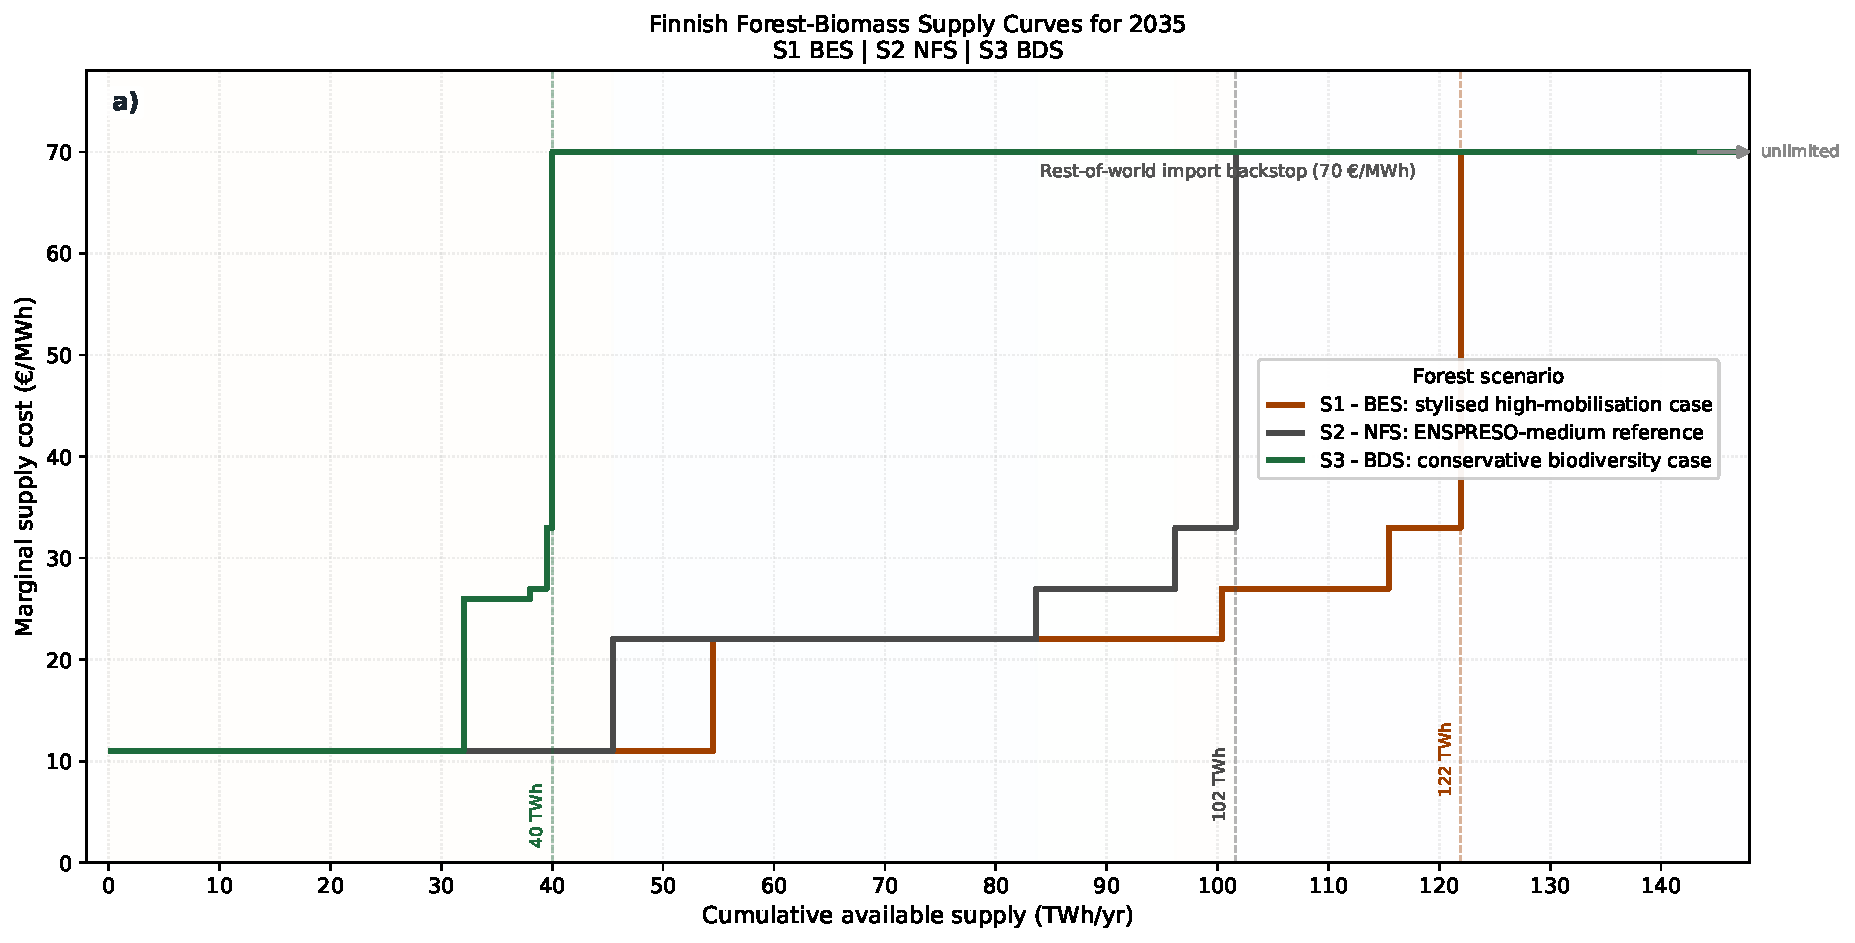
\includegraphics[width=0.98\linewidth]{biomass_supply_curves_fi_2035.pdf}
  \caption{Finnish forest-biomass supply curves used in the 2035 scenario matrix. S1 is a stylised high-biomass sensitivity bound (+20\% above the ENSPRESO medium 2035 baseline), S2 the ENSPRESO-medium reference, and S3 a conservative biodiversity-constrained case revised against \citet{blattertSectoralPoliciesCause2022}, \citet{monkkonenEcologicallyEconomicallySustainable2024}, and recent Finnish national wood-energy statistics \citep{Luke2025ForestTrade}.}
  \label{fig:fi_biomass_supply_curve}
\end{figure}


Figure~\ref{fig:fi_biomass_supply_curve} presents the three scenario supply curves as classical stepwise cost ladders (cumulative available supply on the horizontal axis, marginal cost on the vertical axis). Several features are worth highlighting. All three curves share the cheapest step (\texttt{WOOD\_FI1}: industrial by-products at 11~€/MWh), the least sensitive to forest governance choices because it originates from existing processing plant by-products rather than additional harvesting decisions. Their capacities differ, however, reflecting how much industrial residue each narrative mobilises: 54.5~TWh in S1/BES, 45.4~TWh in S2/NFS, and 32.0~TWh in S3/BDS (Table~\ref{tab:fi_biomass_capacities}). After FI1, the three scenarios diverge sharply. S3/BDS exhausts its domestic ceiling at 40~TWh after only three further small steps -- logging residues (6.0~TWh at 26~€/MWh), secondary woodchips (1.5~TWh at 27~€/MWh), and fuelwood (0.5~TWh at 33~€/MWh) -- then immediately jumps to the Baltic/Nordic import backstop at 70~€/MWh: a price discontinuity of more than 40~€/MWh with no intermediate domestic option. By contrast, S2/NFS extends through four domestic steps up to 101.5~TWh before reaching the backstop, and S1/BES reaches 122.0~TWh. This horizontal compression of the S3 curve illustrates a key modelling insight: biodiversity-constrained forest management does not simply reduce the quantity of cheap biomass while leaving the merit order intact -- it eliminates intermediate cost steps entirely and makes the energy system abruptly dependent on expensive imports once the domestic ceiling is reached. The cost consequences of the constraint therefore manifest primarily as a price jump rather than a gradual cost increase, which is why tight forest-biomass ceilings interact strongly with ambitious GHG targets: the optimiser has no moderately priced margin to exploit and must substitute toward other low-carbon options or accept the high-cost import step. Two limitations matter in particular. First, the RED~II-derived GHG values in Table~\ref{tab:fi_biomass_ladder} (FI1: 10, FI3: 14, FI4: 19~tCO$_2$eq/GWh) replace a preliminary monotone gradient (20, 24, 26) used in an earlier development version. The correction is downward for FI1, FI3, and FI4 because mill-gate and industrial wood residues have shorter supply chains than in-forest collected logging residues. These revised values are implemented in the model input files used for all scenario runs in this paper. A key clarification is that the model's GHG constraint acts on net combustion CO$_2$ only; supply-chain emissions are tracked and reported but not separately constrained by the policy budget. The supply-chain correction therefore does not affect optimised system costs, forest-wood quantities, or qualitative technology-substitution results. Second, because the Belgian low-quality share constraint is not yet reintroduced, the Finnish first stage is stronger on transparent supply ranking than on physical feedstock-quality constraints. For the present paper, this keeps the focus on how domestic forest biomass availability changes across management narratives, but future work should strengthen the feedstock-quality treatment.


\\\\
The retained forward-looking analysis uses a completed $3 \times 3$ scenario matrix. The forest dimension consists of S1/BES, S2/NFS, and S3/BDS. The policy dimension consists of an unconstrained case, a -95\% GHG case, and a -95\% GHG case with full nuclear phase-out. The completed runs show that the unconstrained 2035 system is already strongly decarbonised, whereas the conservative S3 case immediately saturates its 40~TWh ceiling under the -95\% target and therefore removes forest biomass as a flexible adjustment margin.


This paper reports the calibrated 2017 benchmark, the static 2035 forest-biomass ladder, and the completed forest-by-GHG scenario matrix. Disturbance shocks (windthrow, bark-beetle outbreaks, wildfire, salvage wood pulses, and dynamic price shocks) remain future work and are treated as the logical continuation of the present study rather than as implemented results.

\section{Results}
\label{sec:results}

\subsection{Finland 2017 Validation}

To establish model credibility before turning to forward-looking scenarios, the Finnish implementation of EnergyScope was calibrated against a historical baseline year. The reference run uses 12 typical days and relaxes the CO$_2$ emission cap to avoid a non-physical forced-CCS artefact in the historical reproduction. The purpose of this benchmark is not to claim predictive validation of the future, but to test whether a constrained historical configuration can reproduce the known structure of the Finnish 2017 energy system with acceptable deviations.


Table~\ref{tab:fi_validation_2017} summarises the main indicators of the calibrated benchmark against the Finnish 2017 reference values. The main result is that the model reproduces the overall primary-energy balance, electricity mix, and net CO$_2$ emissions with high fidelity. All major primary-energy aggregates except solar remain within about $\pm 5\%$, electricity imports and CHP generation are also close to the statistical reference, and total net CO$_2$ emissions are reproduced almost exactly.

This agreement is also visible in Figure~\ref{fig:fi_validation_main}, which provides the two main graphical validation checks retained in the paper. The left panel shows that the model reproduces the dominant Finnish 2017 primary-energy pillars, especially biomass, oil, gas, coal and nuclear, without requiring large compensating errors across fuels. The right panel shows that the electricity balance is also captured at the right order of magnitude, with the main remaining deviation concentrated in gas-based generation rather than in the low-carbon backbone of nuclear, hydro and wind.

Two residual mismatches should nevertheless be discussed explicitly. First, district-heating production is overestimated by 43.4\%. This is not primarily a calibration failure but a structural aggregation artefact: in the present EnergyScope formulation, the district-heating share is applied to the full low-temperature heat pool, including industrial low-temperature demand, whereas Finnish statistics mainly report residential and service-sector network heat. Second, gas-fired electricity remains 36.7\% above the statistical reference because district-heating CHP in the model produces electricity as an unavoidable by-product when gas is routed through CHP technologies. These limitations do not invalidate the historical benchmark, but they define the clearest remaining structural aggregation issues.

\begin{table}[H]
  \centering
  \small
  \renewcommand{\arraystretch}{1.08}
  \begin{tabularx}{\linewidth}{llrrr}
    \toprule
    \textbf{Category} & \textbf{Indicator} & \textbf{Actual 2017} & \textbf{Model} & \textbf{Error} \\
    \midrule
    Primary energy & Biomass & 100.0 & 96.8 & -3.2\% \\
    Primary energy & Oil & 82.0 & 80.9 & -1.4\% \\
    Primary energy & Gas & 20.0 & 20.0 & 0.0\% \\
    Primary energy & Coal + peat & 35.0 & 35.0 & 0.0\% \\
    Primary energy & Nuclear & 65.0 & 65.1 & +0.1\% \\
    Primary energy & Hydro & 15.0 & 14.6 & -2.7\% \\
    Primary energy & Wind & 5.0 & 4.8 & -4.1\% \\
    Electricity & CHP & 20.73 & 20.49 & -1.2\% \\
    Electricity & Gas power & 3.2 & 4.37 & +36.7\% \\
    Electricity & Imports & 20.43 & 19.54 & -4.4\% \\
    Heat & District-heating production & 36.5 & 52.33 & +43.4\% \\
    Emissions & CO$_2$ & 41.2 & 41.25 & +0.1\% \\
    \bottomrule
  \end{tabularx}
  \caption{Main indicators of the calibrated Finland 2017 benchmark against the statistical reference system. Primary energy and electricity values are in TWh; CO$_2$ emissions in MtCO$_2$/y.}
  \label{tab:fi_validation_2017}
\end{table}

\begin{figure}[H]
  \centering
  \begin{minipage}{0.49\linewidth}
    \centering
    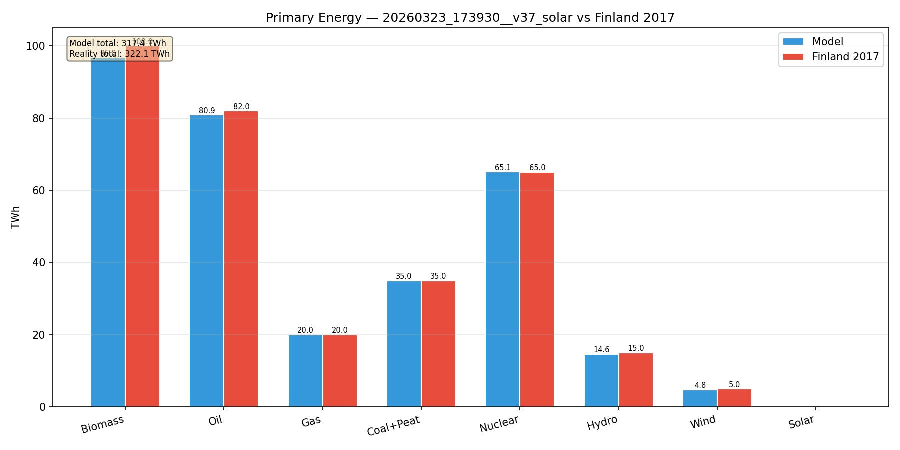
\includegraphics[width=\linewidth]{validation_2017_pe_comparison.pdf}
  \end{minipage}
  \hfill
  \begin{minipage}{0.49\linewidth}
    \centering
    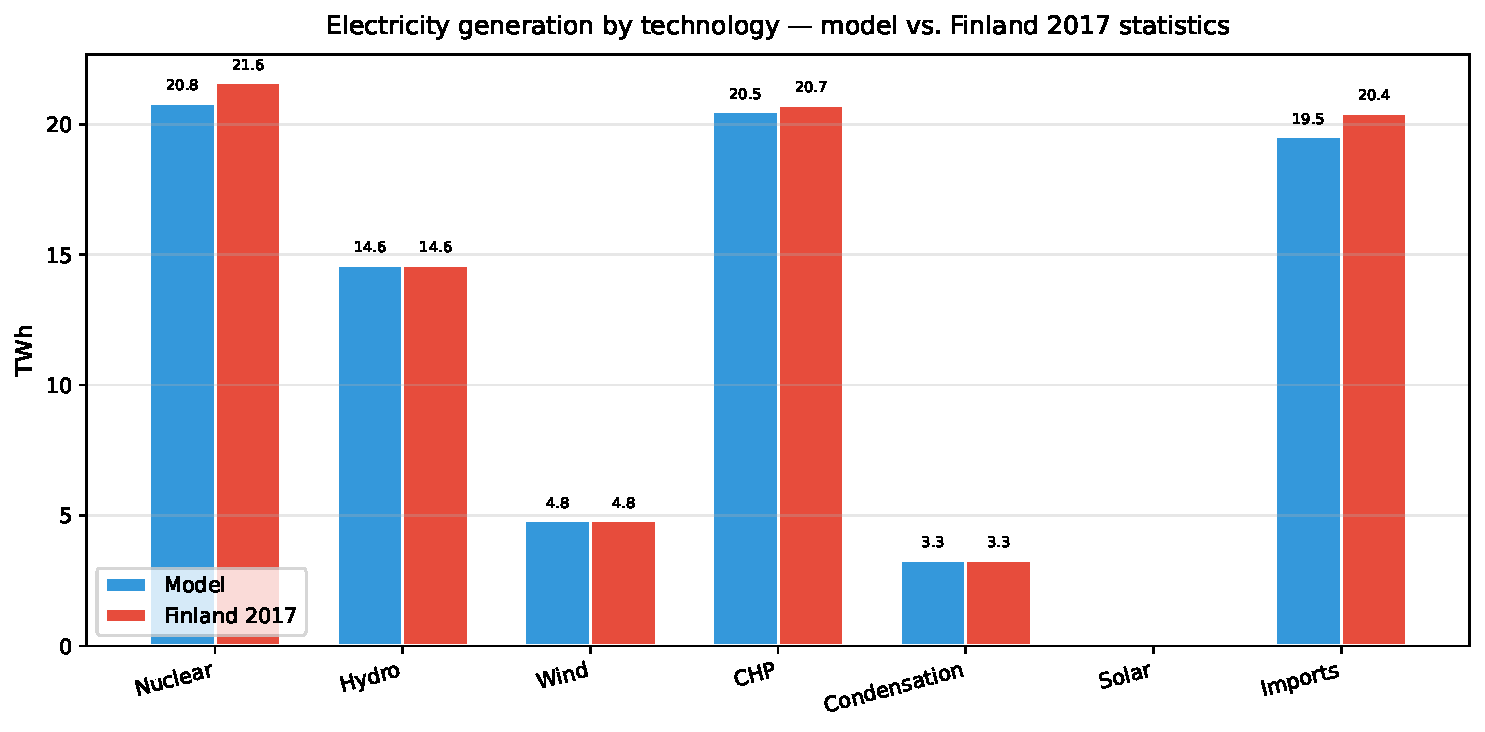
\includegraphics[width=\linewidth]{validation_2017_elec_comparison.pdf}
  \end{minipage}
  \caption{Finland 2017 validation: model versus Statistics Finland. Left: primary energy supply by carrier (TWh). Right: electricity generation by technology (TWh). The main residual deviations are discussed in the text.}
  \label{fig:fi_validation_main}
\end{figure}

For the main text, the retained validation visuals are therefore limited to the primary-energy comparison, the electricity-generation comparison, and a structural Sankey view of the calibrated system. Figure~\ref{fig:fi_validation_sankey} complements Figure~\ref{fig:fi_validation_main} by showing that the calibrated benchmark is not only numerically close to Finnish statistics but also structurally coherent as an integrated energy system. In particular, the corrected heat-pump branch makes clear that low-temperature heat is produced from a combination of electricity and ambient heat, while the broader diagram highlights the expected roles of nuclear and hydro in electricity supply, lignocellulosic biomass in heat and CHP, and oil products in mobility and non-energy uses.

\begin{figure}[H]
  \centering
  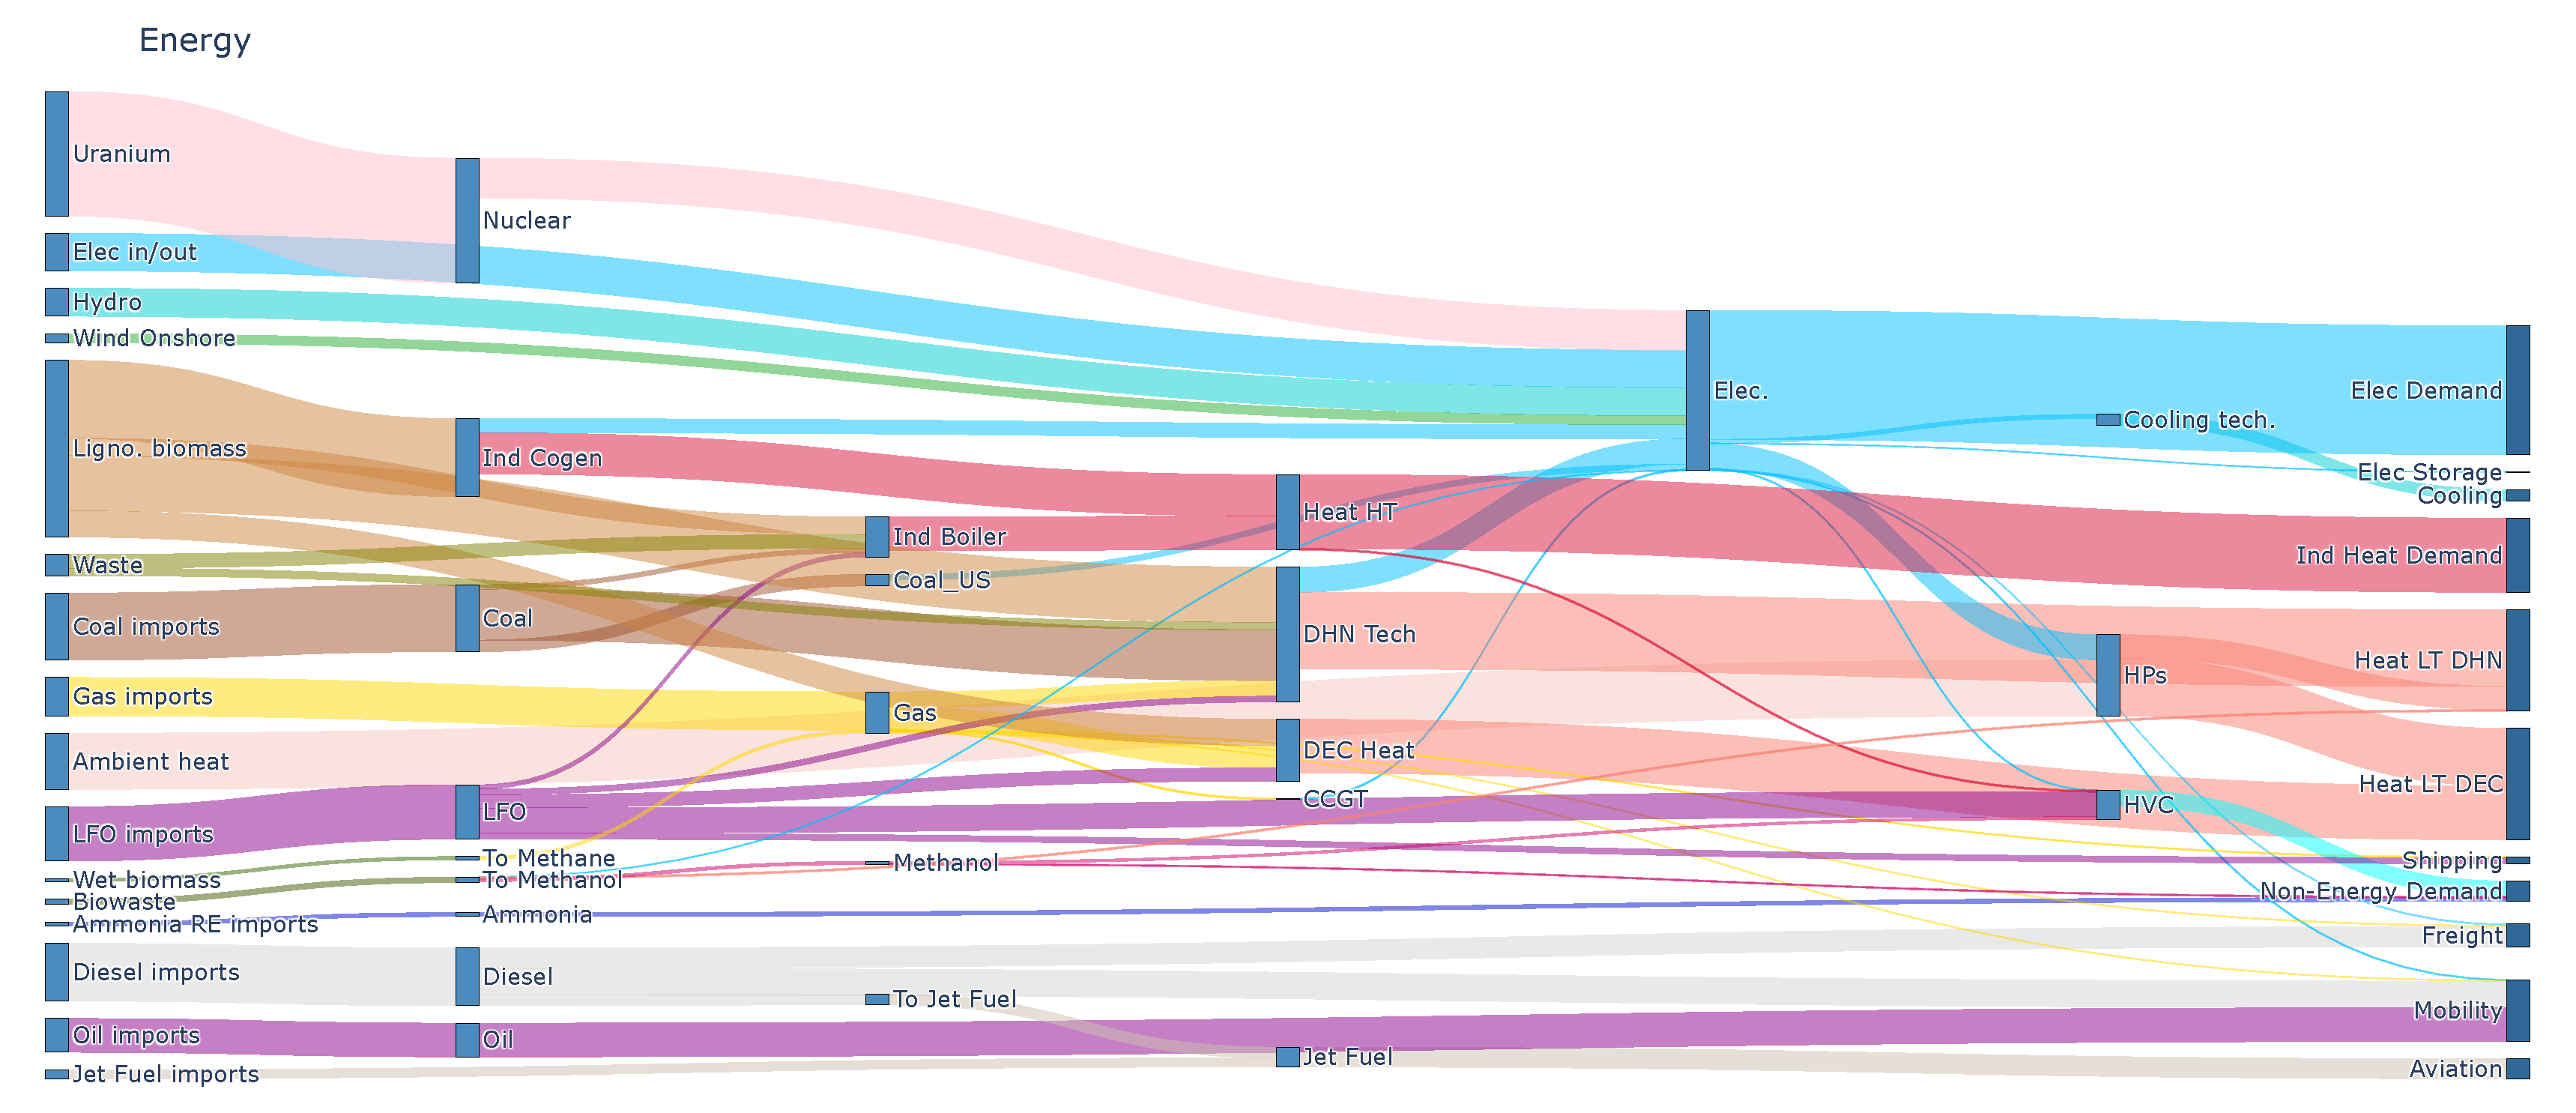
\includegraphics[width=\linewidth]{validation_2017_sankey.pdf}
  \caption{Structural Sankey view of the modelled energy mix for Finland 2017}
  \label{fig:fi_validation_sankey}
\end{figure}

\subsection{Finland 2035 Results Under Forest and Emissions Scenarios}

The forward-looking analysis uses the completed $3 \times 3$ matrix crossing three forest-biomass supply narratives (S1/BES, S2/NFS, S3/BDS) with three policy configurations (unconstrained, -95\% GHG with nuclear, and -95\% GHG with full nuclear phase-out). Across the three forest cases, the unconstrained 2035 optimum already yields net CO$_2$ emissions between about 12.6 and 13.1~MtCO$_2$/y, corresponding to roughly 68--70\% reduction relative to 2017. The policy-relevant question is therefore not whether the unconstrained 2035 system decarbonises, but how the last part of the path toward a -95\% target changes when forest biomass becomes scarce and nuclear is removed.

\begin{table}[H]
  \centering
  \small
  \renewcommand{\arraystretch}{1.08}
  \begin{tabularx}{\linewidth}{llrrr}
    \toprule
    \textbf{Forest scenario} & \textbf{Policy case} & \textbf{Cost} & \textbf{CO$_2$ net} & \textbf{Forest wood used} \\
    \midrule
    S1/BES & Unconstrained & 22.40 bnEUR/y & 13.02 Mt/y & 54.5 TWh \\
    S1/BES & -95\% GHG (with nuclear) & 22.92 bnEUR/y & 2.06 Mt/y & 74.2 TWh \\
    S1/BES & -95\% GHG (nuclear phase-out) & 22.94 bnEUR/y & 2.06 Mt/y & 100.4 TWh \\
    S2/NFS & Unconstrained & 22.46 bnEUR/y & 12.57 Mt/y & 45.4 TWh \\
    S2/NFS & -95\% GHG (with nuclear) & 23.02 bnEUR/y & 2.06 Mt/y & 74.2 TWh \\
    S2/NFS & -95\% GHG (nuclear phase-out) & 23.12 bnEUR/y & 2.06 Mt/y & 96.2 TWh \\
    S3/BDS & Unconstrained & 22.62 bnEUR/y & 13.10 Mt/y & 32.0 TWh \\
    S3/BDS & -95\% GHG (with nuclear) & 23.56 bnEUR/y & 2.06 Mt/y & 40.0 TWh \\
    S3/BDS & -95\% GHG (nuclear phase-out) & 23.90 bnEUR/y & 2.06 Mt/y & 40.0 TWh \\
    \bottomrule
  \end{tabularx}
  \caption{Summary of the retained Finland 2035 forest-biomass scenario matrix. Forest-wood use sums the Finnish forest-biomass ladder resources only.}
  \label{tab:fi_2035_matrix}
\end{table}

Table~\ref{tab:fi_2035_matrix} summarises the main results of the retained scenario matrix. Three patterns deserve emphasis. First, the unconstrained cases are relatively close in annualised system cost, but they already differ in biomass use: S3/BDS is more constrained than S1 and S2 even without a climate target. A structural detail worth noting is that in all three unconstrained cases the model saturates exactly the first supply-ladder step (WOOD\_FI1, cheap industrial by-products) and draws nothing from the higher-cost domestic steps, indicating that the 2035 Finnish energy demand without a climate target can be met entirely from the cheapest biomass fractions; the supply-curve design therefore matters primarily under the stringent GHG constraint. Second, the -95\% case with nuclear fully saturates the conservative S3 ceiling while leaving headroom in S1 and S2. Third, removing nuclear substantially increases biomass demand in S1 and S2 (from 74.2~TWh to 100.4~TWh in S1, and to 96.2~TWh in S2), yet the additional system cost is surprisingly small: only 0.02 and 0.10~bn~EUR/y respectively, because the additional wood is available at the intermediate steps of an unconstrained supply ladder. By contrast, S3 cannot expand further because its 40~TWh domestic ceiling is already binding, making the nuclear phase-out more costly (0.34~bn~EUR/y additional). In other words, S3 does not make deep decarbonisation infeasible in the optimiser, but it removes forest biomass as a flexible adjustment margin and therefore becomes the highest-cost configuration, with a sensitivity to nuclear availability roughly three times greater than in S1.
\begin{figure}[H]
  \centering
  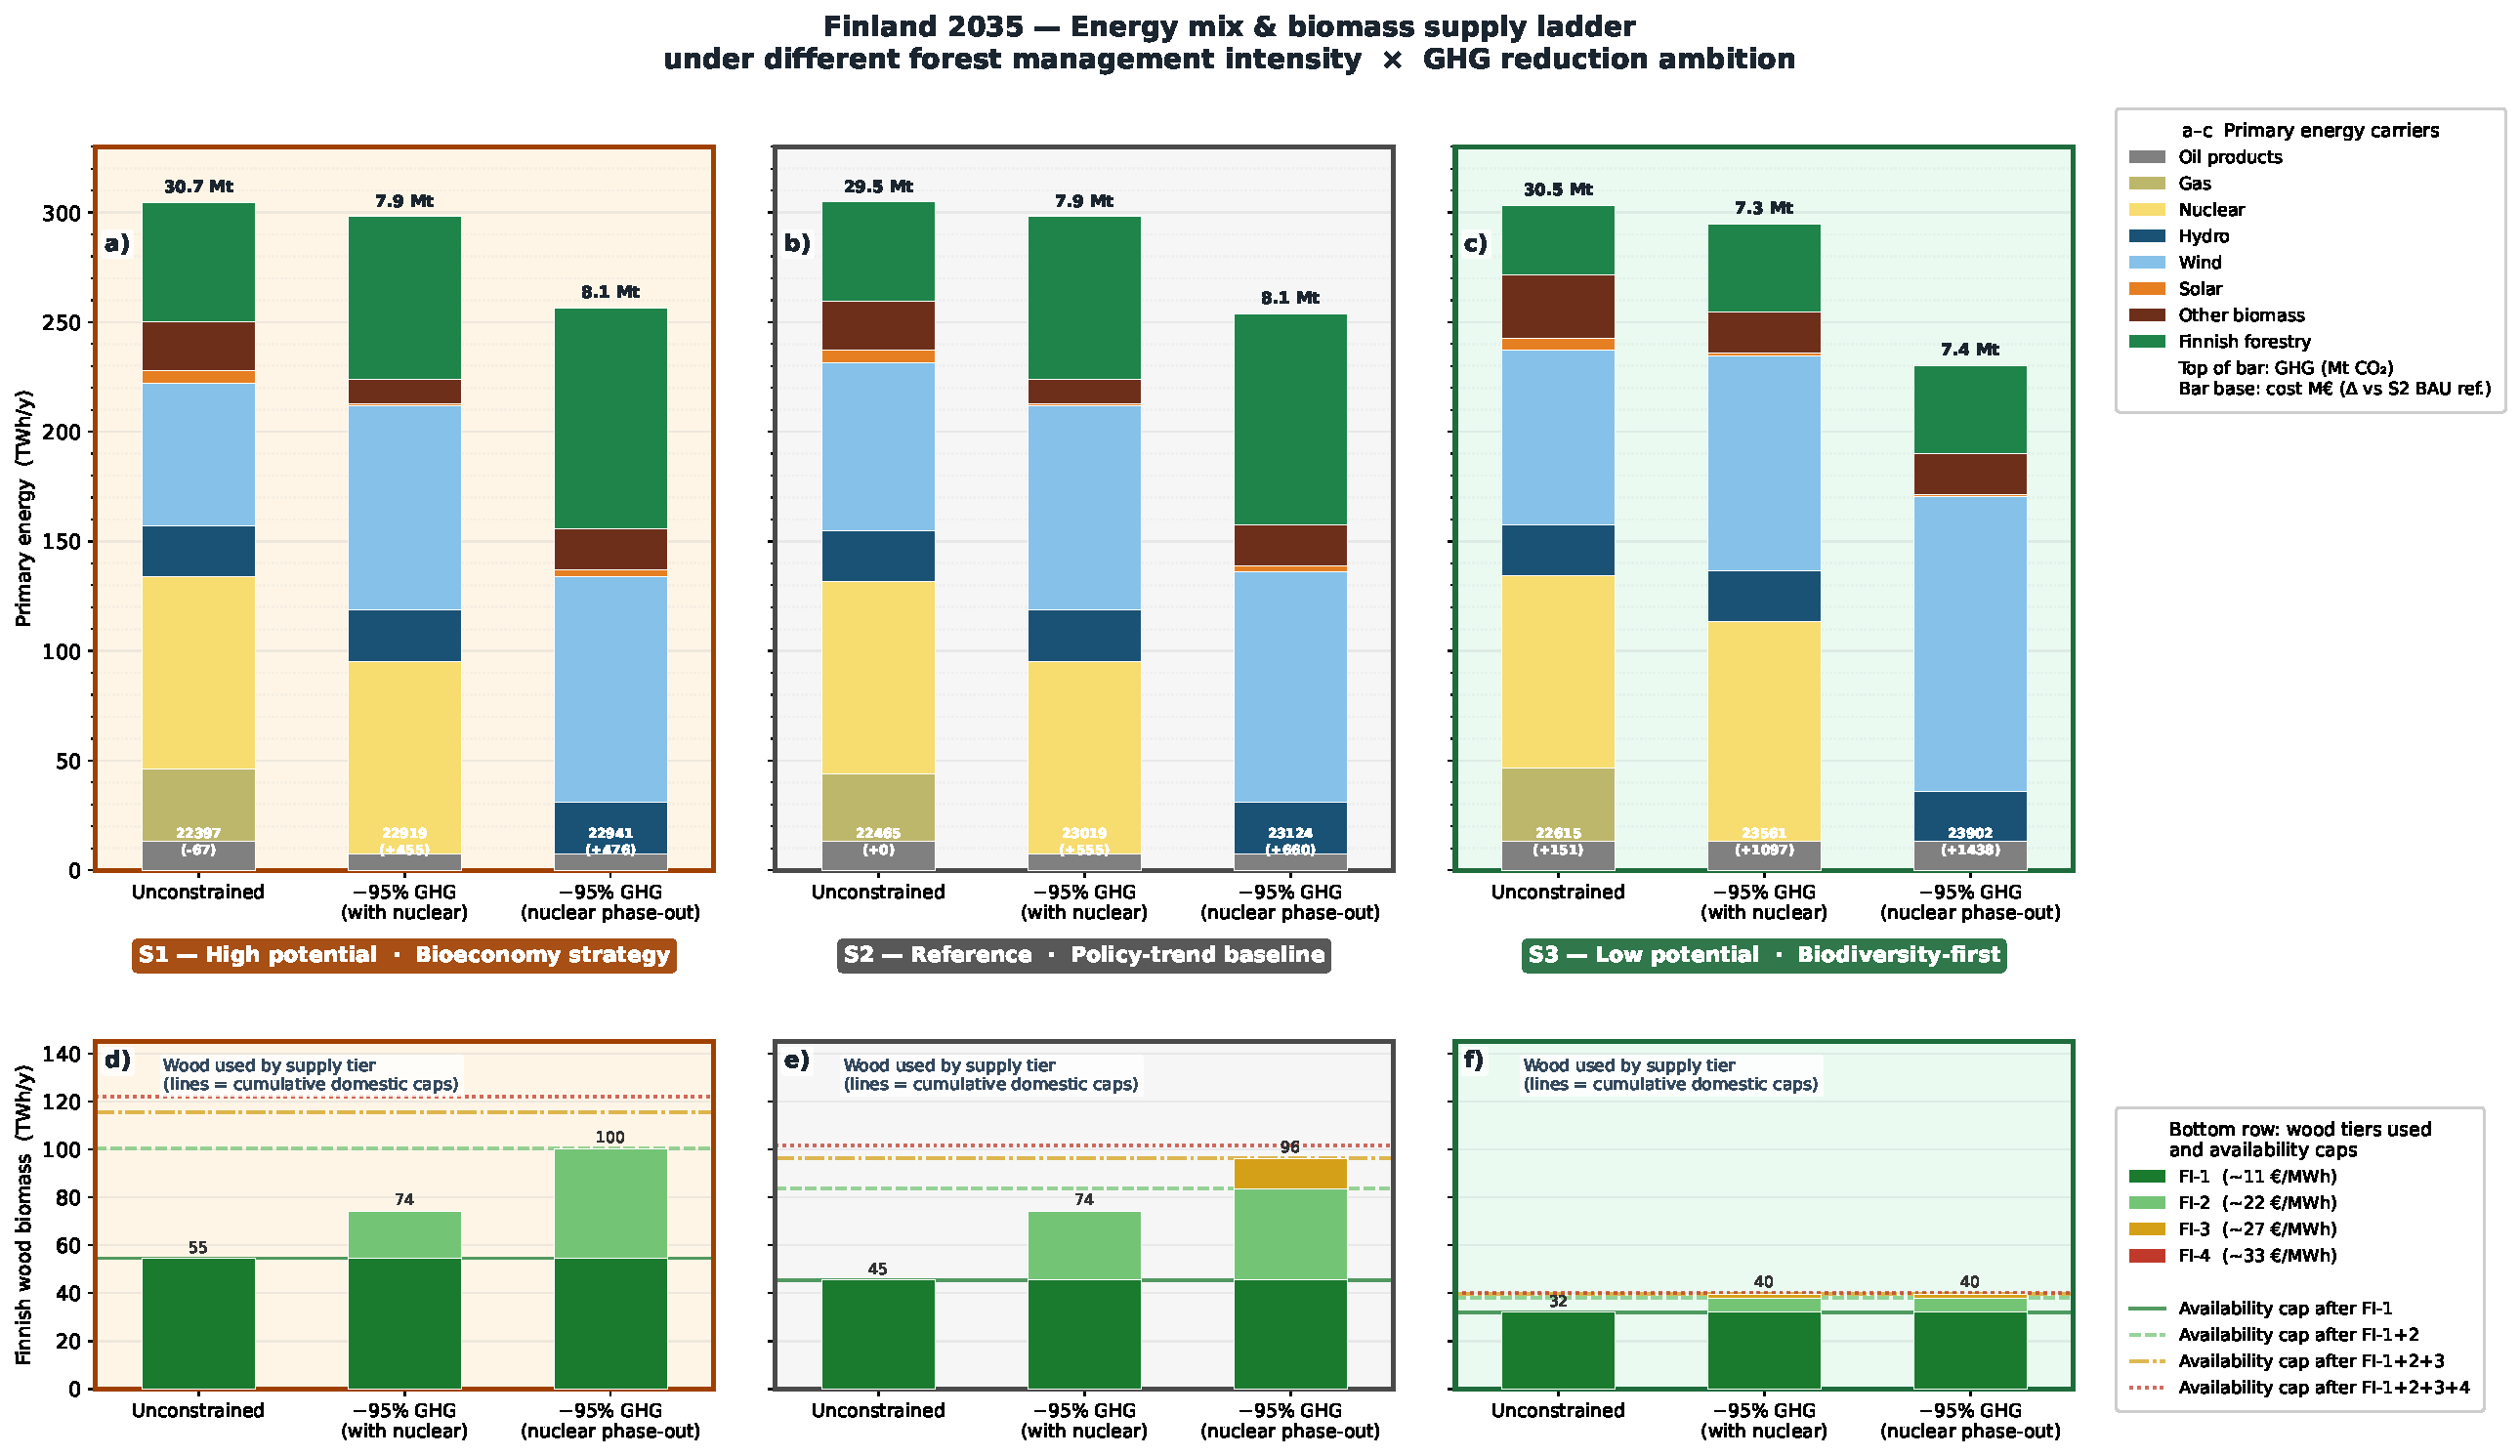
\includegraphics[width=\linewidth]{forest_scenarios_2035_energy_matrix.pdf}
  \caption{Finland 2035 scenario matrix across three forest-management cases and three GHG configurations. The top row shows the primary-energy mix, while the bottom row shows the use of the Finnish forest-wood supply ladder. The unconstrained cases already reach roughly a 70\% reduction versus 2017, while the biodiversity-constrained S3 case is distinguished by early saturation of the domestic wood ceiling under the -95\% target.}
  \label{fig:fi_2035_energy_matrix}
\end{figure}
These system-level shifts are easier to read in Figure~\ref{fig:fi_2035_energy_matrix}. The top row shows that the main transition from the unconstrained cases to the -95\% cases is not a simple linear reduction in fossil use, but a reconfiguration of the entire primary-energy mix around electricity, nuclear availability, and scarce biomass: fossil imports fall from roughly 46--47~TWh to about 8~TWh across all three forest cases, a reduction of more than 80\%, while additional renewables and biomass fill the gap. The bottom row shows that in the unconstrained cases only the cheapest FI1 step (industrial by-products) is mobilised, whereas the -95\% cases unlock the next supply tier -- FI2 logging residues add 19.6~TWh in S1, 28.7~TWh in S2, and S3 activates all four domestic steps to reach its 40~TWh ceiling. The no-nuclear variants push further up the ladder in S1 (FI2 nearly exhausted at 45.9~TWh) and into the FI3 step in S2 (adding 12.5~TWh). This is the key result of the scenario exercise: biodiversity-constrained forest supply does not prevent deep decarbonisation in the model, but it removes cheap domestic biomass as an adjustment margin precisely when the climate constraint becomes stringent.

\begin{figure}[H]
  \centering
  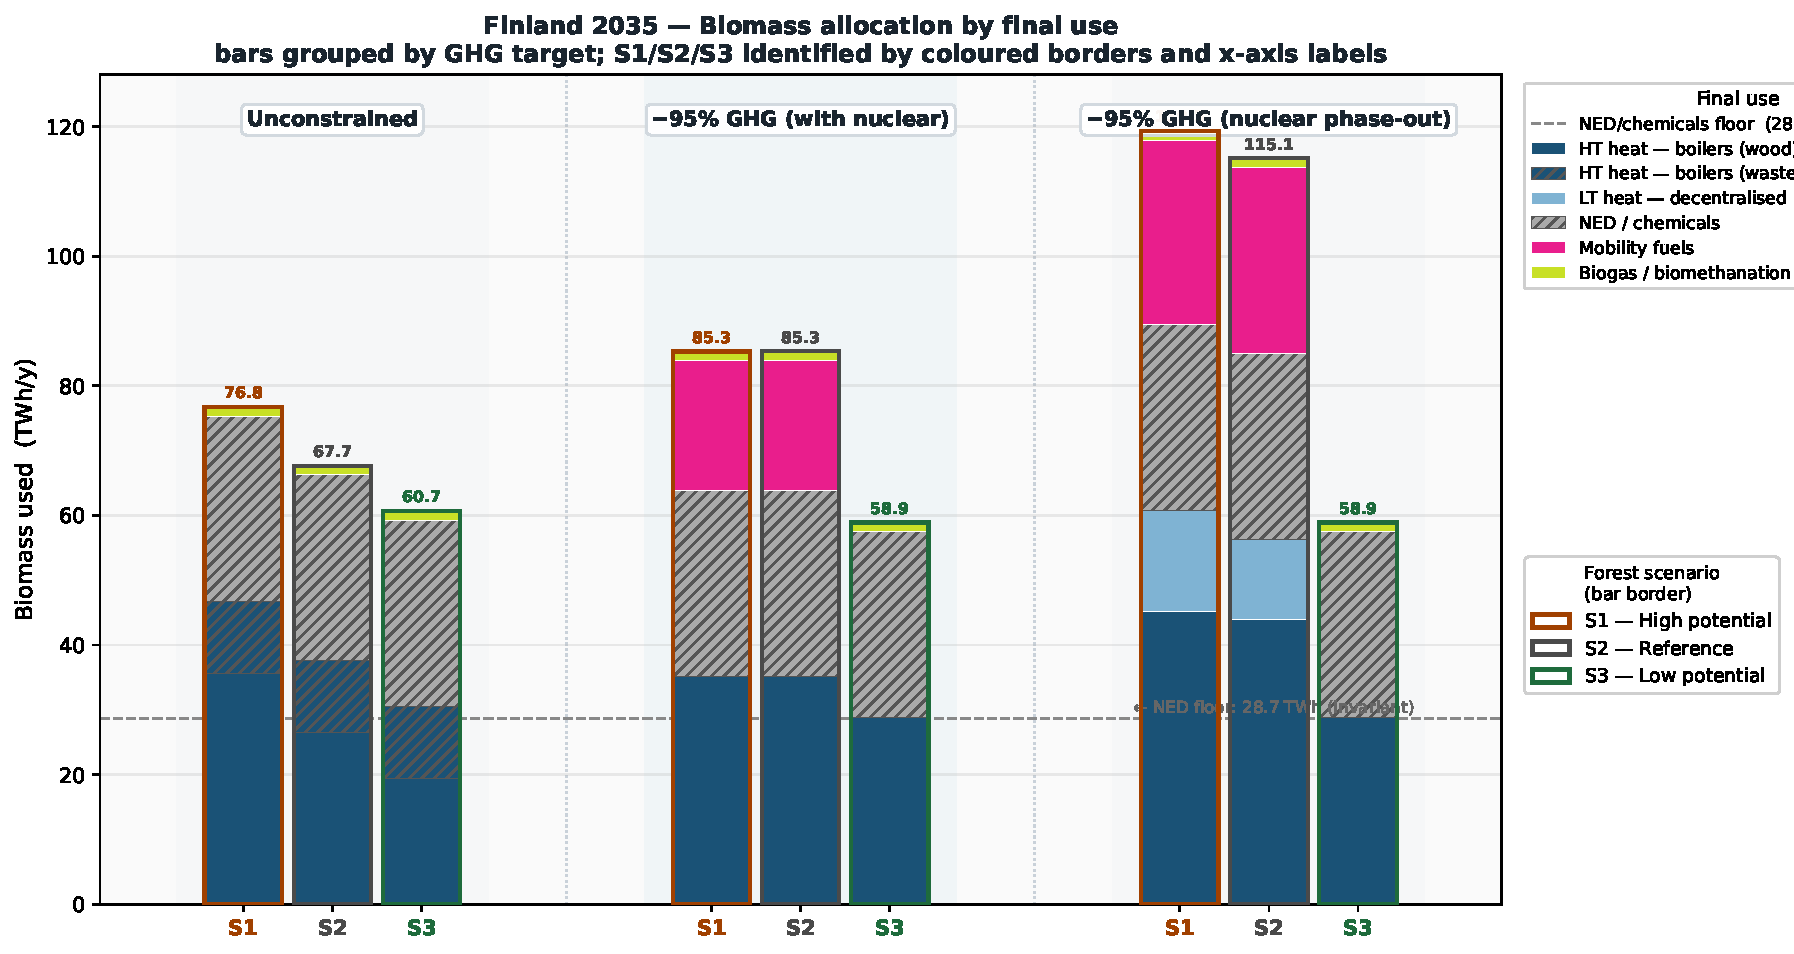
\includegraphics[width=\linewidth]{forest_scenarios_2035_biomass_allocation.pdf}
  \caption{Biomass allocation by final use in Finland 2035. The figure highlights how the no-nuclear cases increase pressure on biomass in S1 and S2, whereas S3/BDS remains capped by its conservative forest-biomass ceiling and therefore relies more heavily on non-biomass adjustments elsewhere in the system.}
  \label{fig:fi_2035_biomass_allocation}
\end{figure}

Figure~\ref{fig:fi_2035_biomass_allocation} adds the end-use interpretation behind that aggregate picture. Three patterns stand out.

First, roughly 27.9~TWh is directed to high-value-chemicals production and approximately 0.8~TWh to methanol synthesis across all nine scenarios -- a near-constant baseline driven by exogenous non-energy industrial demand that the optimiser cannot reroute. This commitment means that the full S3/BDS ceiling of 40~TWh retains only about 12~TWh for heat or transport use after chemicals are satisfied.

Second, the -95\% GHG constraint triggers a qualitative shift in S1/BES and S2/NFS. In the unconstrained cases the residual wood after chemicals is directed almost entirely to industrial process-heat boilers (25.9~TWh in S1, 16.8~TWh in S2, and 9.8~TWh in S3). Under the climate target, approximately 20.1~TWh of the available budget in S1 and S2 is instead converted to road diesel and aviation jet fuel -- the hardest-to-electrify end uses -- while industrial-heat allocation remains broadly stable. In S3/BDS, the 40~TWh ceiling is already fully committed to chemicals and industry heat under the climate constraint, leaving no margin for transport biofuels; the transport sector is instead partially decarbonised through imported renewable diesel, substituting the domestic biomass-to-fuel conversion route with a higher-cost import pathway.

Third, removing nuclear in S1/BES and S2/NFS amplifies biomass pressure across multiple services simultaneously. Beyond transport biofuels (which remain near 20~TWh), the model deploys an additional 15.6~TWh (S1) and 12.4~TWh (S2) through decentralised building-heat boilers, an additional 10.1~TWh (S1) and 8.8~TWh (S2) through industrial-heat boilers, and a new 8.3--8.6~TWh allocation to synthetic methane for seasonal storage and industrial gas demand. The result is that, in the absence of nuclear baseload, biomass becomes a multi-service strategic resource simultaneously filling gaps in building heat, industrial heat, gas supply, and transport fuels. S3/BDS cannot follow this pattern: its end-use breakdown is structurally identical between the -95\% and the no-nuclear case because the 40~TWh domestic ceiling is already binding under the weaker constraint. The additional decarbonisation burden -- decentralised heat, synthetic gas -- must be absorbed entirely by non-biomass pathways, which is why the cost penalty for nuclear removal is nearly three times larger in S3 than in S1.

The policy implication is therefore not only about the total quantity of forest biomass available, but about which end-use priorities the forest budget can still accommodate once both biodiversity constraints and nuclear policy choices tighten simultaneously.

\subsection{Next steps: disturbance shocks and dynamic biomass supply}

The present paper deliberately stops at static 2035 management scenarios. The next stage of the research is to couple the Finnish forest simulator used by the Jyvaskyla/LUKE team with the FLAM and PICUS disturbance modules developed in the ForestNavigator framework, so that annual biomass supply curves can respond to wildfire risk, bark-beetle outbreaks, windthrow, salvageable calamity wood, and the subsequent reduction in standing stock \citep{venalainenClimateChangeInduces2020,hlasnyDevastatingOutbreakBark2021,tothImpactsCalamityLogging2020}. In energy-system terms, this would extend the current forest scenarios from fixed 2035 ladders to time-varying biomass availability and cost trajectories under contrasting management regimes and climate pathways.

The concept-note design is not simply a lower biomass ceiling. It is intended to capture three mechanisms that are absent from the current paper: a short-lived calamity-wood pulse after a disturbance event, quality and marginal-cost changes for salvage biomass, and a medium-term decline in future harvestable stock after damaged cohorts are depleted \citep{tothImpactsCalamityLogging2020,reckaRoleBiomassDecarbonisation2023}. Methodologically, the proposed extension uses a pre-shock 2030 EnergyScope snapshot, followed by a post-shock snapshot with limited re-optimisation in order to reflect realistic investment lead times for biomass CHP, DHN extensions, and other inherited infrastructure. The disturbance module is therefore presented as the logical next research phase built on the present article: the current paper establishes the calibrated national baseline and the static forest-scenario framework, while the coupled forest-disturbance workflow would add dynamic timing, quality, and price effects on top of that validated base.


\section{Conclusion}
\label{sec:conclusion}

This paper develops a first national EnergyScope TD application for Finland centred on the role of forest biomass in a 2035 transition setting. By translating contested forest-management narratives into explicit biomass supply curves, it links the Finnish forest-policy debate to whole-energy-system optimisation. The calibrated 2017 benchmark shows that the model can reproduce the main Finnish primary-energy aggregates, electricity balance, and net CO$_2$ emissions with high fidelity, while keeping the remaining structural mismatches transparent, especially for district heating and gas-related CHP co-production. This validation step is essential because it establishes that the Finnish implementation is sufficiently credible for scenario exploration before moving to forward-looking policy questions.

For the 2035 scenario matrix, the central result is not that biodiversity-constrained forest management makes deep decarbonisation impossible, but that it removes forest biomass as a low-cost adjustment margin exactly when climate ambition becomes stringent. The unconstrained 2035 cases are already strongly decarbonised, whereas the -95\% cases reveal much sharper competition for biomass, particularly when nuclear is removed. S1/BES and S2/NFS retain some flexibility to expand forest-wood use, but S3/BDS saturates its conservative 40~TWh ceiling and becomes the highest-cost configuration. The paper therefore shows that forest-biomass assumptions are not a secondary sensitivity: they materially shape the cost and allocation logic of deep decarbonisation in Finland. The next research step is to extend this validated static framework toward disturbance-driven annual biomass supply trajectories, so that wind, beetle, and wildfire shocks can be studied within the same energy-system optimisation framework.





\bibliographystyle{plainnat}
\bibliography{references}

\end{document}